\documentclass[12pt,a4paper]{report}

% ==============================================================================
% GÓI VÀ ĐỊNH DẠNG TÀI LIỆU (PACKAGES & FORMATTING)
% ==============================================================================
\usepackage[utf8]{inputenc}
\usepackage[vietnamese]{babel}
\usepackage[margin=2.5cm]{geometry}
\usepackage{amsmath,amssymb,amsfonts}
\usepackage{graphicx}
\usepackage{booktabs}
\usepackage{multirow}
\usepackage{float}
\usepackage{hyperref}
\usepackage{caption}
\usepackage{subcaption}
\usepackage{fancyhdr}
\usepackage{setspace}
\usepackage{listings}
\usepackage{xcolor}

\setstretch{1.3}

\hypersetup{
    colorlinks=true,
    linkcolor=blue!80!black,
    citecolor=green!60!black,
    urlcolor=blue!90!black
}

\graphicspath{{../figures/}}

% Thiết lập header/footer
\pagestyle{fancy}
\fancyhf{}
\fancyhead[L]{\small Đề tài 14: Dự đoán khách hàng hủy đặt phòng khách sạn}
\fancyhead[R]{\small Nhập môn Học máy (2026--2027)}
\fancyfoot[C]{\thepage}

\lstset{
    basicstyle=\ttfamily\small,
    backgroundcolor=\color{gray!10},
    frame=single,
    breaklines=true,
    keywordstyle=\color{blue}\bfseries,
    commentstyle=\color{green!50!black},
    stringstyle=\color{red!70!black}
}

% ==============================================================================
% PHẦN MỞ ĐẦU (TITLE & PREAMBLE)
% ==============================================================================
\begin{document}

\begin{titlepage}
    \centering
    \vspace*{1cm}
    {\Large\bfseries BỘ GIÁO DỤC VÀ ĐÀO TẠO}\\[0.5cm]
    {\large\bfseries TRƯỜNG ĐẠI HỌC CÔNG NGHỆ}\\[2cm]
    
    {\Huge\bfseries BÁO CÁO BÀI TẬP LỚN}\\[0.5cm]
    {\Large\bfseries HỌC PHẦN: NHẬP MÔN HỌC MÁY}\\[0.3cm]
    {\large Năm học: 2026 -- 2027}\\[2cm]
    
    \fbox{
        \parbox{0.9\textwidth}{
            \centering\vspace{0.5cm}
            {\LARGE\bfseries ĐỀ TÀI 14}\\[0.3cm]
            {\Large\bfseries DỰ ĐOÁN KHÁCH HÀNG HỦY ĐẶT PHÒNG KHÁCH SẠN}\\[0.2cm]
            {\large\textit{(Hotel Booking Cancellation Prediction)}}\vspace{0.5cm}
        }
    }\\[2.5cm]
    
    \begin{flushleft}
        \large
        \textbf{Nhóm sinh viên thực hiện:} Nhóm 3 thành viên\\
        \textbf{1.} Thành viên 1 -- \textit{Phụ trách Khám phá dữ liệu (EDA)}\\
        \textbf{2.} Thành viên 2 -- \textit{Phụ trách Tiền xử lý \& Huấn luyện mô hình}\\
        \textbf{3.} Thành viên 3 -- \textit{Phụ trách Đánh giá, Phân tích lỗi \& Báo cáo}\\[0.8cm]
        \textbf{Giảng viên hướng dẫn:} Giảng viên phụ trách môn học
    \end{flushleft}
    
    \vfill
    {\large Hà Nội, Năm 2026}
\end{titlepage}

\pagenumbering{roman}
\tableofcontents
\newpage
\listoffigures
\newpage
\listoftables
\newpage

\pagenumbering{arabic}

% ==============================================================================
% CÁC CHƯƠNG NỘI DUNG (CHAPTERS)
% ==============================================================================
\chapter{ĐẶT VẤN ĐỀ VÀ PHÂN TÍCH YÊU CẦU}

\section{Giới thiệu đề tài}
Trong bối cảnh nền kinh tế dịch vụ và du lịch phát triển mạnh mẽ trên phạm vi toàn cầu, ngành quản trị khách sạn và lưu trú đóng vai trò trụ cột. Đề tài 14: \textbf{``Dự đoán khách hàng hủy đặt phòng khách sạn (Hotel Booking Cancellation Prediction)''} được nghiên cứu nhằm áp dụng các kỹ thuật học máy có giám sát (Supervised Machine Learning) vào việc dự đoán khả năng khách hàng hủy phòng ngay từ thời điểm đặt phòng.

\section{Bối cảnh và ý nghĩa bài toán}
Phòng khách sạn là loại hàng hóa có hạn sử dụng ngắn hạn (Perishable Inventory) -- một đêm phòng nếu không được bán sẽ mất đi giá trị vĩnh viễn và không thể thu hồi. Khi khách hàng hủy đặt phòng đột ngột:
\begin{itemize}
    \item Doanh thu dự kiến bị sụt giảm nghiêm trọng.
    \item Khách sạn bị lãng phí nguồn lực chuẩn bị (nhân lực buồng phòng, thực phẩm).
    \item Nếu khách sạn áp dụng chiến lược đặt phòng vượt mức (Overbooking) quá cao mà không có mô hình định lượng, nguy cơ thiếu phòng sẽ gây ảnh hưởng tiêu cực đến uy tín thương hiệu.
\end{itemize}
Mô hình học máy dự báo sớm nguy cơ hủy giúp nhà quản trị tối ưu hóa kế hoạch kinh doanh và chính sách định giá động.

\section{Mục tiêu nghiên cứu}
\begin{enumerate}
    \item Khám phá và phân tích sâu các nhân tố ảnh hưởng đến quyết định hủy phòng từ dữ liệu thực tế.
    \item Thiết kế hai phương án tiền xử lý: Pipeline A (Cơ bản) và Pipeline B (Cải tiến với Kỹ thuật đặc trưng) đảm bảo tuyệt đối không xảy ra rò rỉ dữ liệu (No Data Leakage).
    \item Triển khai, tối ưu hóa và so sánh hiệu quả của các thuật toán: Baseline (DummyClassifier), K-Nearest Neighbors (KNN), Decision Tree (Cây quyết định).
    \item Đánh giá toàn diện mô hình trên tập kiểm thử độc lập thông qua nhiều chỉ số: Accuracy, Precision, Recall, F1-Score, ROC-AUC và phân tích ma trận nhầm lẫn.
    \item Thực hiện phân tích lỗi (False Positive và False Negative) nhằm đưa ra khuyến nghị thực tiễn cho nhà quản trị khách sạn.
\end{enumerate}

\section{Đối tượng nghiên cứu}
Đối tượng nghiên cứu là các giao dịch đặt phòng khách sạn được lưu vết trong hệ thống thông tin quản lý, bao gồm các thông tin về khách hàng, thời gian đặt trước, loại phòng, hình thức đặt cọc, số lượng khách và các yêu cầu đặc biệt.

\section{Phạm vi nghiên cứu}
Nghiên cứu tập trung vào bài toán Phân loại nhị phân (Binary Classification) với biến mục tiêu \texttt{is\_canceled} $\in \{0, 1\}$. Các dữ liệu trạng thái phát sinh sau khi đơn hàng kết thúc (như \texttt{reservation\_status}) bị loại trừ để bảo đảm tính thực tiễn khi ứng dụng mô hình tại thời điểm nhận đặt phòng.

\section{Giới thiệu bộ dữ liệu Hotel Booking Demand}
Nghiên cứu sử dụng bộ dữ liệu chuẩn mực \textbf{Hotel Booking Demand} của Jesse Mostipak \cite{mostipak2019kaggle}, bắt nguồn từ công trình nghiên cứu của Antonio, de Almeida và Nunes (2019) \cite{antonio2019hotel}.
\begin{itemize}
    \item \textbf{Quy mô:} 119,390 dòng quan sát và 32 thuộc tính.
    \item \textbf{Phạm vi khách sạn:} Gồm hai loại hình: Resort Hotel (H1, vùng Algarve) và City Hotel (H2, thành phố Lisbon, Bồ Đào Nha).
    \item \textbf{Khoảng thời gian:} Dữ liệu ghi nhận từ ngày 01/07/2015 đến ngày 31/08/2017.
\end{itemize}

\section{Mô tả các đặc trưng dữ liệu}
Bộ dữ liệu gồm 31 đặc trưng đầu vào và 1 biến mục tiêu:
\begin{itemize}
    \item \textbf{Đặc trưng thời gian:} \texttt{lead\_time}, \texttt{arrival\_date\_year}, \texttt{arrival\_date\_month}, \texttt{arrival\_date\_week\_number}, \texttt{arrival\_date\_day\_of\_month}, \texttt{stays\_in\_weekend\_nights}, \texttt{stays\_in\_week\_nights}.
    \item \textbf{Đặc trưng khách hàng:} \texttt{adults}, \texttt{children}, \texttt{babies}, \texttt{country}, \texttt{is\_repeated\_guest}, \texttt{customer\_type}.
    \item \textbf{Lịch sử đặt phòng:} \texttt{previous\_cancellations}, \texttt{previous\_bookings\_not\_canceled}, \texttt{booking\_changes}.
    \item \textbf{Đặc trưng thương mại:} \texttt{hotel}, \texttt{meal}, \texttt{market\_segment}, \texttt{distribution\_channel}, \texttt{reserved\_room\_type}, \texttt{assigned\_room\_type}, \texttt{deposit\_type}, \texttt{agent}, \texttt{company}, \texttt{days\_in\_waiting\_list}, \texttt{adr}, \texttt{required\_car\_parking\_spaces}, \texttt{total\_of\_special\_requests}.
\end{itemize}

\section{Phân tích khám phá dữ liệu (EDA)}
Quá trình phân tích khám phá dữ liệu trên toàn bộ 119,390 dòng quan sát đã xác định các đặc điểm phân phối quan trọng:
\begin{itemize}
    \item \textbf{Tỷ lệ hủy phòng theo khách sạn:} City Hotel có tỷ lệ hủy lên đến $41.73\%$ (33,102 đơn hủy trên 79,330 đơn), trong khi Resort Hotel có tỷ lệ hủy là $27.76\%$ (11,122 đơn hủy trên 40,060 đơn).
    \item \textbf{Tác động của hình thức đặt cọc (\texttt{deposit\_type}):} Đáng lưu ý, nhóm đặt cọc không hoàn lại (\texttt{Non Refund}) có tỷ lệ hủy lên tới $99.36\%$ (14,494 đơn hủy trên 14,587 đơn). Đây là các hợp đồng đặt theo đoàn hoặc đại lý mà chính sách buộc ghi nhận trạng thái hủy khi đoàn không đến.
    \item \textbf{Thời gian đặt trước (\texttt{lead\_time}):} Khách đặt trước càng sớm thì tỷ lệ hủy càng cao (đơn đặt trên 1 năm có tỷ lệ hủy trên $70\%$, trong khi đơn đặt trong vòng 1 tuần chỉ có tỷ lệ hủy dưới $15\%$).
    \item \textbf{Yêu cầu đặc biệt (\texttt{total\_of\_special\_requests}):} Khách hàng có từ 2 yêu cầu đặc biệt trở lên có tỷ lệ hủy dưới $22\%$, thấp hơn nhiều so với khách không có yêu cầu nào ($47.7\%$).
\end{itemize}

\begin{figure}[H]
    \centering
    \begin{subfigure}{0.48\textwidth}
        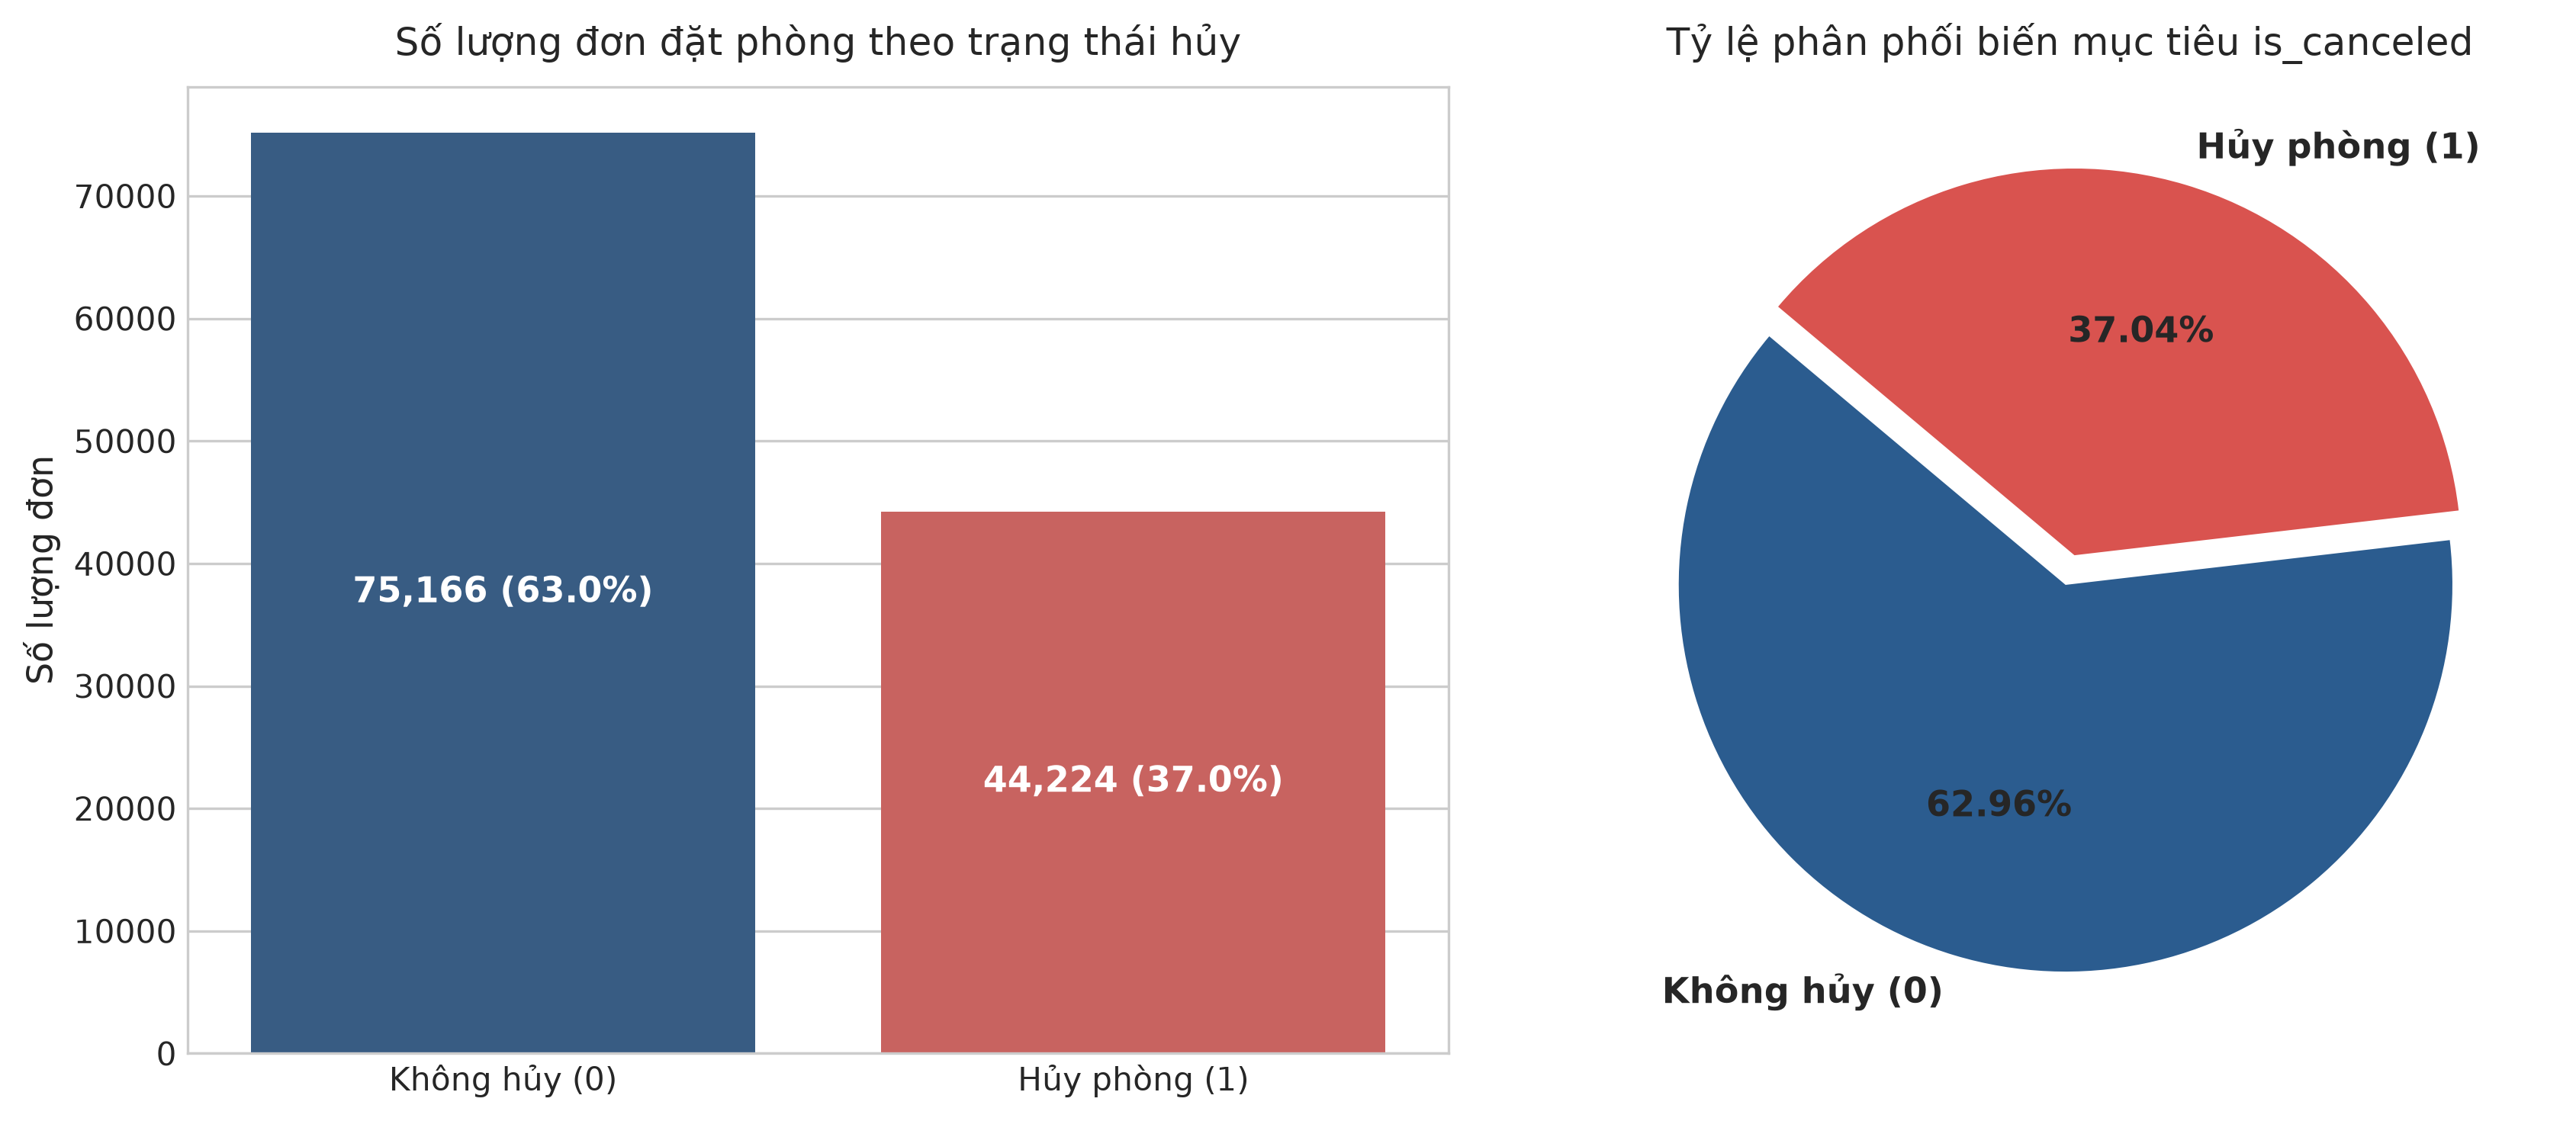
\includegraphics[width=\linewidth]{01_target_distribution.png}
        \caption{Phân phối biến mục tiêu \texttt{is\_canceled}}
    \end{subfigure}
    \begin{subfigure}{0.48\textwidth}
        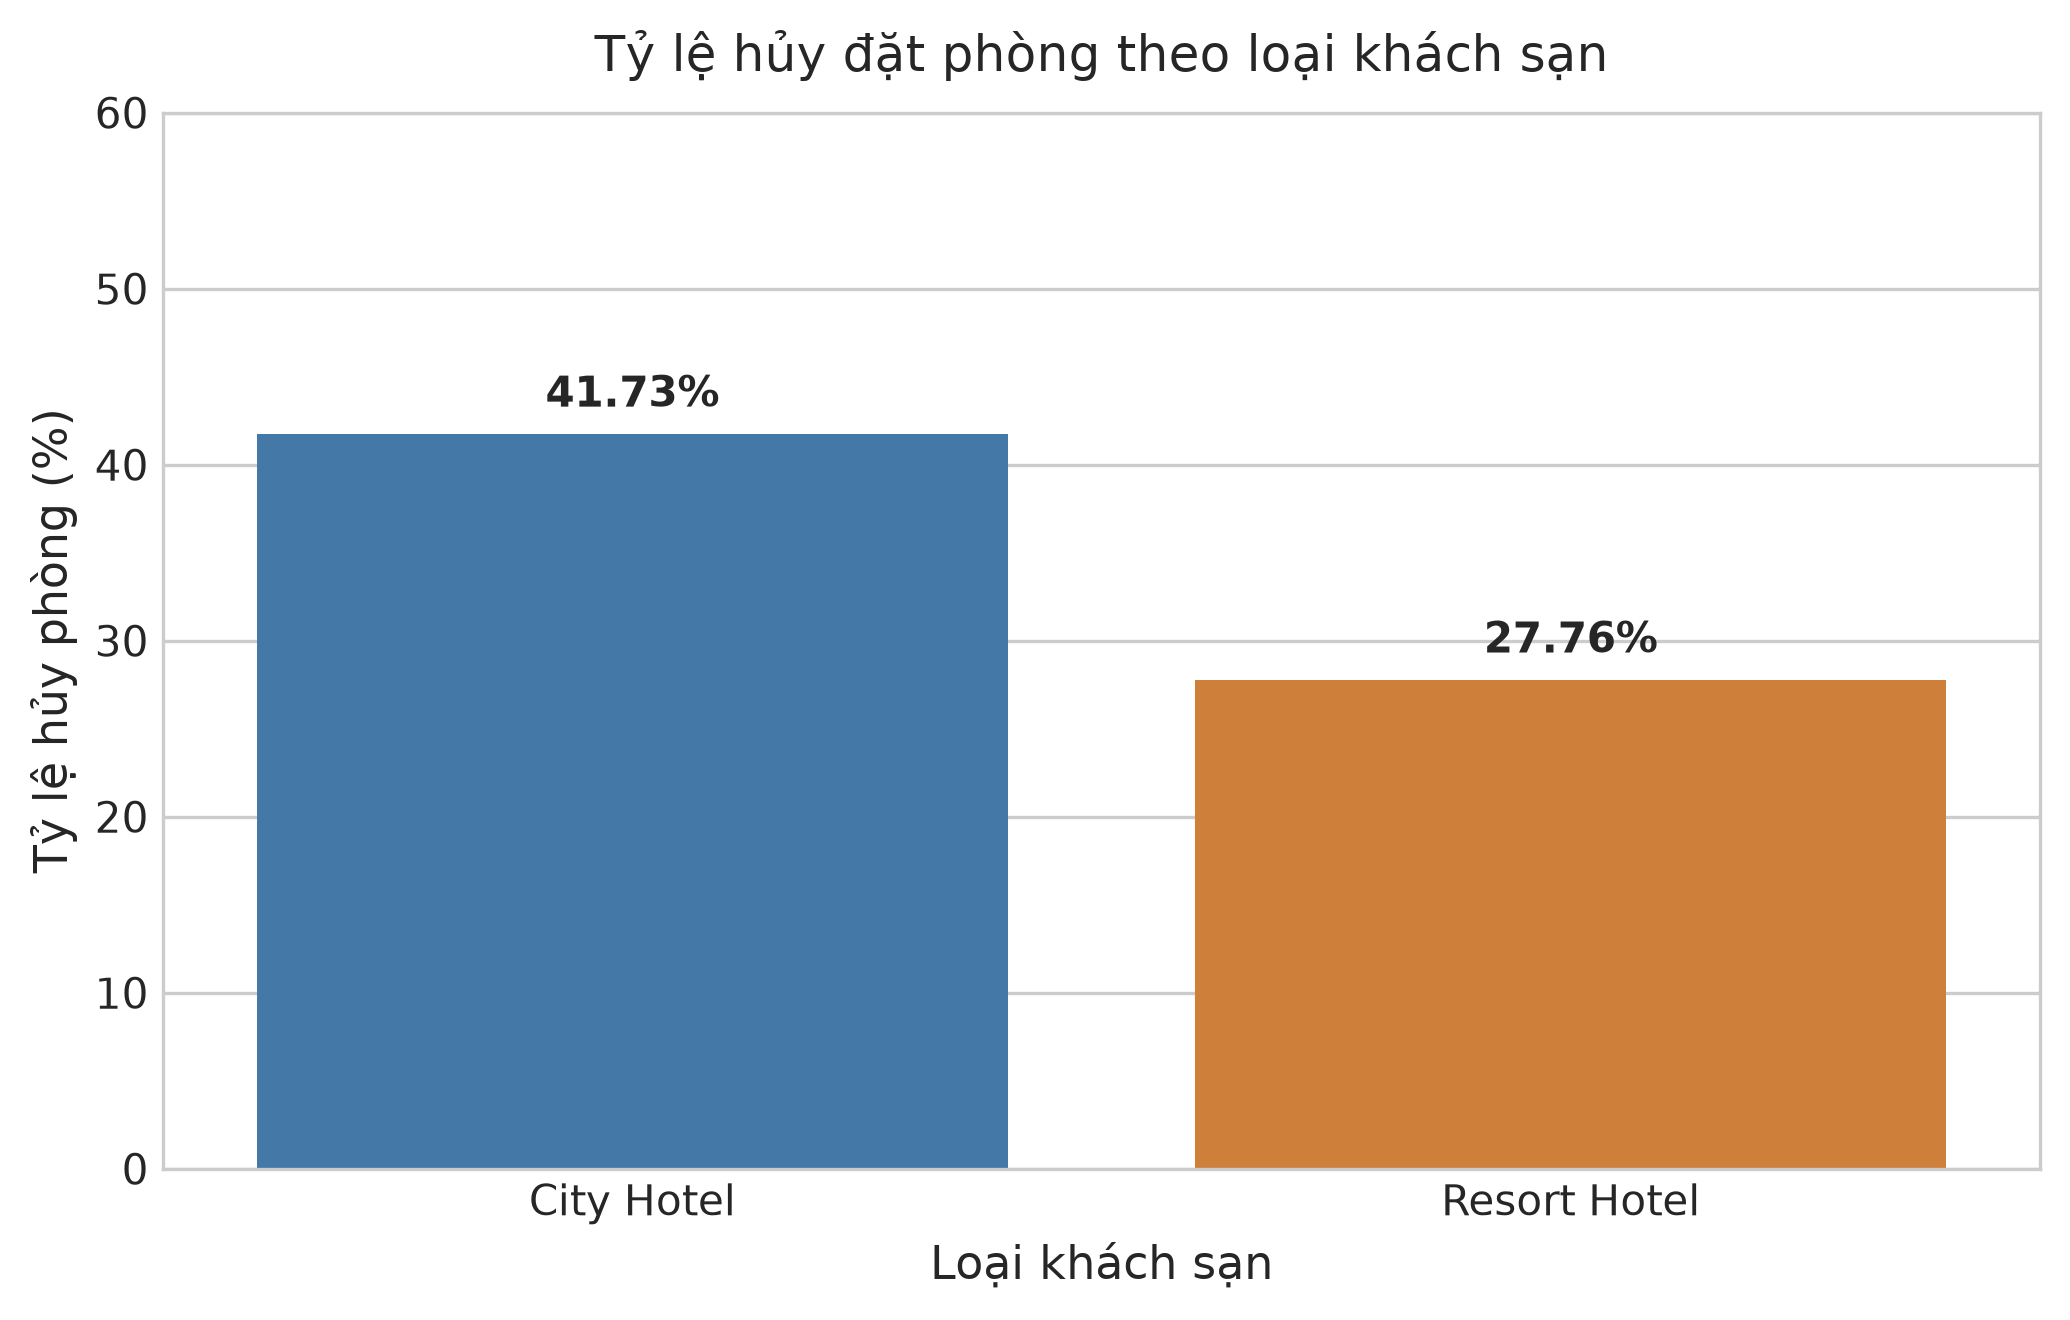
\includegraphics[width=\linewidth]{03_cancellation_by_hotel.png}
        \caption{Tỷ lệ hủy theo loại khách sạn}
    \end{subfigure}
    \caption{Phân tích phân phối mục tiêu và loại hình khách sạn}
    \label{fig:eda_overview}
\end{figure}

\begin{figure}[H]
    \centering
    \begin{subfigure}{0.48\textwidth}
        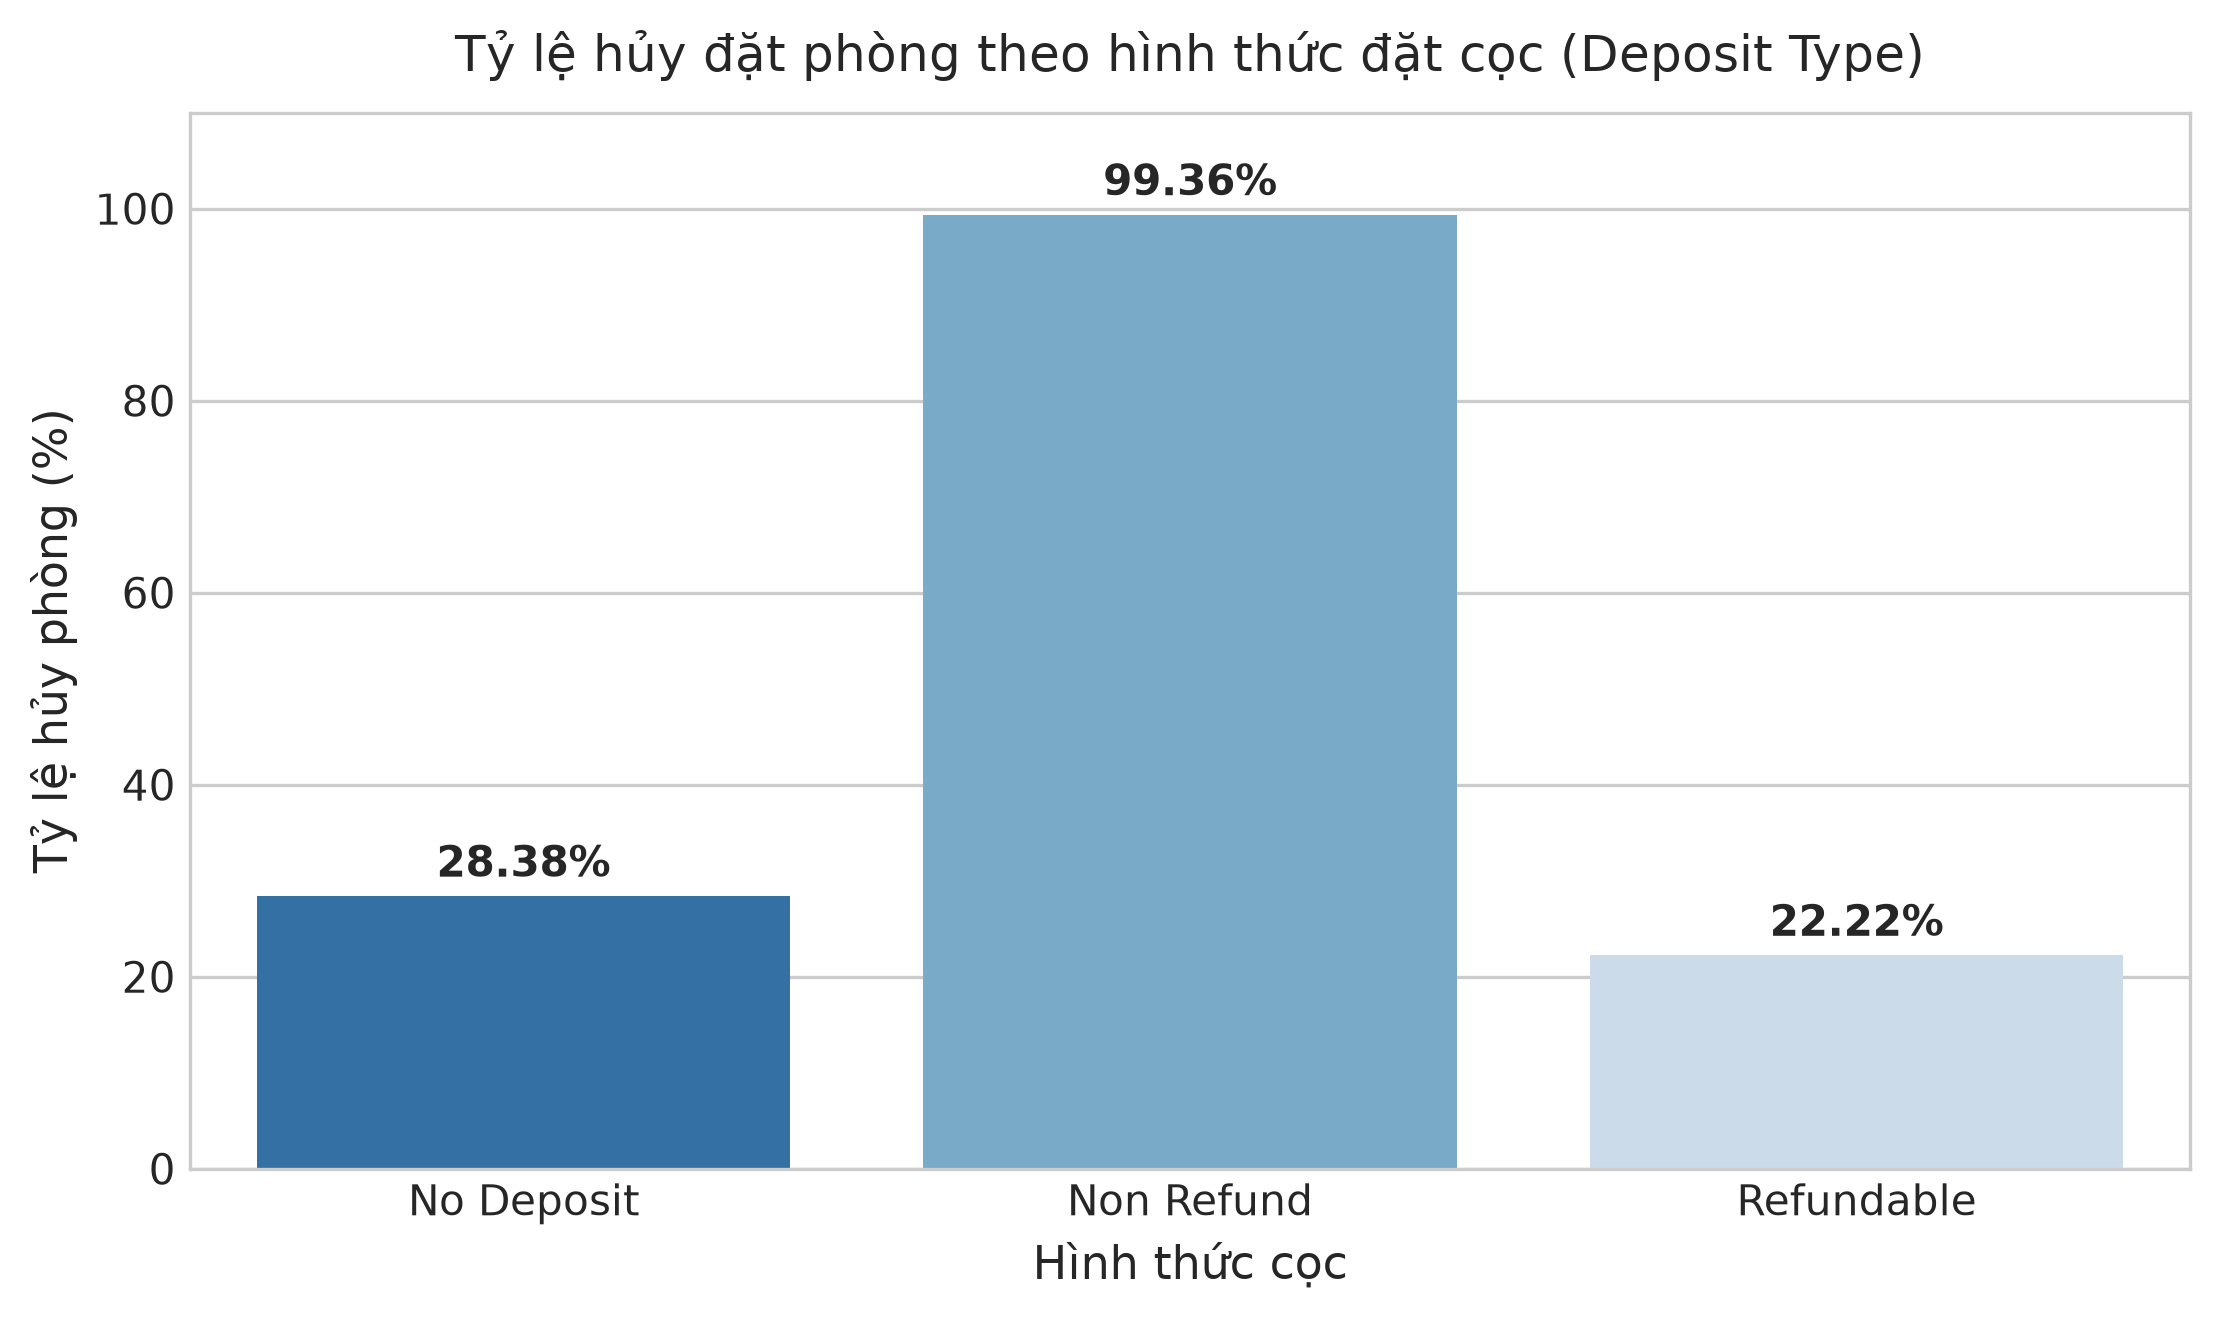
\includegraphics[width=\linewidth]{04_cancellation_by_deposit_type.png}
        \caption{Tỷ lệ hủy theo hình thức đặt cọc}
    \end{subfigure}
    \begin{subfigure}{0.48\textwidth}
        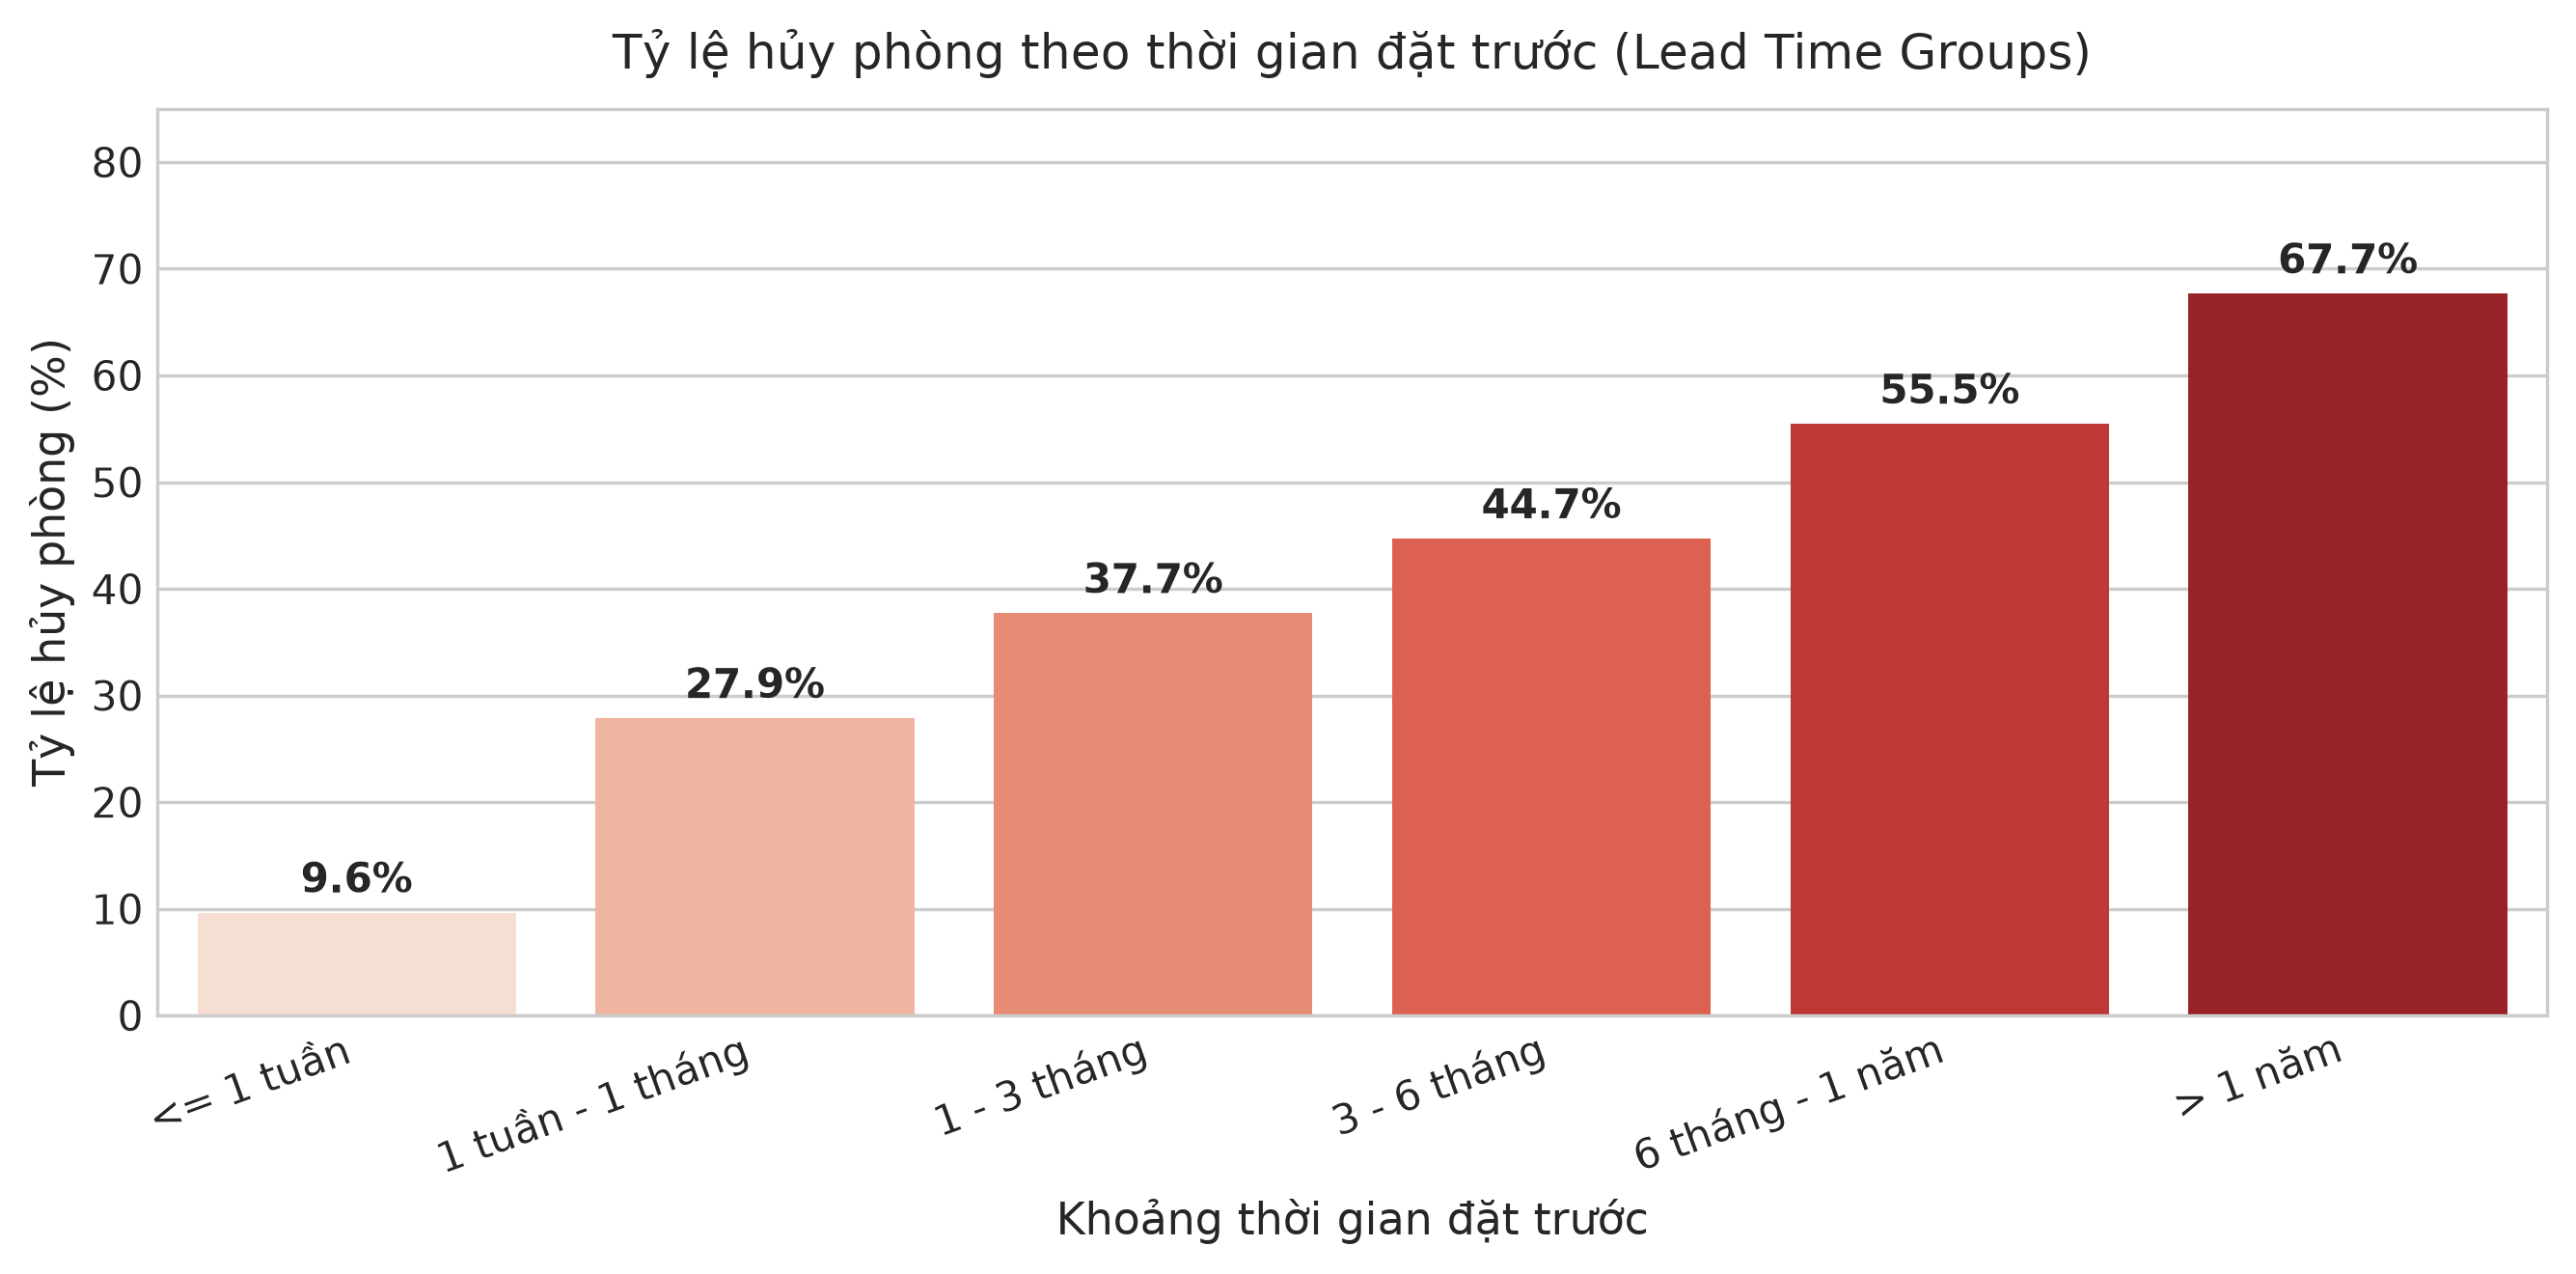
\includegraphics[width=\linewidth]{07_cancellation_by_lead_time_group.png}
        \caption{Tỷ lệ hủy theo khoảng thời gian đặt trước}
    \end{subfigure}
    \caption{Mối quan hệ giữa đặt cọc, thời gian đặt trước và nguy cơ hủy phòng}
    \label{fig:eda_relationships}
\end{figure}

\section{Phân tích biến mục tiêu}
Biến mục tiêu \texttt{is\_canceled} có phân phối thực tế như sau:
\begin{itemize}
    \item Lớp 0 (Khách nhận phòng, không hủy): 75,166 mẫu, chiếm $62.96\%$.
    \item Lớp 1 (Khách hủy phòng hoặc No-Show): 44,224 mẫu, chiếm $37.04\%$.
\end{itemize}
Bộ dữ liệu có độ mất cân bằng nhẹ (tỷ lệ xấp xỉ $1.7 : 1$). Do đó, việc chia dữ liệu cần sử dụng kỹ thuật Stratified Split, và việc đánh giá mô hình không thể chỉ dựa vào Accuracy mà bắt buộc phải sử dụng Precision, Recall và F1-Score.

\section{Các vấn đề phát hiện từ dữ liệu}
\begin{enumerate}
    \item \textbf{Dữ liệu thiếu (Missing Data):}
    \begin{itemize}
        \item \texttt{company}: Thiếu 112,593 giá trị ($94.31\%$).
        \item \texttt{agent}: Thiếu 16,340 giá trị ($13.69\%$).
        \item \texttt{country}: Thiếu 488 giá trị ($0.41\%$).
        \item \texttt{children}: Thiếu 4 giá trị ($0.003\%$).
    \end{itemize}
    \item \textbf{Dữ liệu trùng lặp:} 31,994 dòng ($26.8\%$) có giá trị các thuộc tính trùng nhau hoàn toàn do không có trường định danh cá nhân (ID). Nhóm giữ nguyên tập dữ liệu này để phản ánh đúng phân phối tần suất đặt phòng ngoài thực tế.
    \item \textbf{Giá trị ngoại lệ và dị thường:} Phát hiện 1 dòng có giá phòng trung bình $\text{ADR} = -5.4$ và 180 dòng có tổng số khách bằng 0 (\texttt{adults} + \texttt{children} + \texttt{babies} = 0).
    \item \textbf{Nguy cơ rò rỉ dữ liệu (Data Leakage):} Hai cột \texttt{reservation\_status} và \texttt{reservation\_status\_date} chứa thông tin sau khi giao dịch kết thúc, bắt buộc phải loại bỏ trước khi xây dựng mô hình.
\end{enumerate}

\chapter{THIẾT KẾ GIẢI PHÁP VÀ QUY TRÌNH HỌC MÁY}

\section{Sơ đồ quy trình học máy tổng quát}
Quy trình xây dựng mô hình học máy trong dự án tuân theo tiêu chuẩn công nghiệp:
\begin{enumerate}
    \item \textbf{Data Ingestion \& Validation:} Nạp dữ liệu từ CSV, kiểm tra schema và loại trừ các cột rò rỉ.
    \item \textbf{Train/Test Splitting:} Phân chia dữ liệu có bảo toàn tỷ lệ nhãn (Stratified Split).
    \item \textbf{Preprocessing Pipelines:} Đóng gói các biến đổi dữ liệu bên trong \texttt{ColumnTransformer}.
    \item \textbf{Model Training \& Tuning:} Huấn luyện mô hình và đánh giá chéo 5-fold trên tập Train.
    \item \textbf{Independent Evaluation:} Kiểm thử mô hình trên tập Test độc lập.
    \item \textbf{Diagnostic Error Analysis:} Phân tích các trường hợp dự đoán sai để rút ra giải pháp nghiệp vụ.
\end{enumerate}

\section{Phương pháp chia dữ liệu}
Để phản ánh chính xác hiệu năng mô hình trên dữ liệu chưa từng biết:
\begin{itemize}
    \item Dữ liệu được chia theo tỷ lệ: \textbf{80\% Train} (95,512 mẫu) và \textbf{20\% Test} (23,878 mẫu).
    \item Sử dụng \texttt{stratify=y} để tỷ lệ hủy phòng ở cả hai tập đạt đúng $37.04\%$.
    \item Cố định \texttt{random\_state = 42} để đảm bảo tính tái lập (Reproducibility).
    \item Tập Test được cách ly hoàn toàn và chỉ sử dụng ở khâu đánh giá cuối cùng.
\end{itemize}

\section{Xử lý dữ liệu thiếu}
\begin{itemize}
    \item \textbf{Biến số:} Sử dụng \texttt{SimpleImputer(strategy='median')}. Trung vị (Median) được lựa chọn do các biến số (như \texttt{children}) có phân phối lệch phải mạnh, không bị ảnh hưởng bởi ngoại lệ như giá trị trung bình (Mean).
    \item \textbf{Biến phân loại:} 
    \begin{itemize}
        \item Trong Pipeline A: Điền giá trị xuất hiện nhiều nhất (\texttt{most\_frequent}).
        \item Trong Pipeline B: Điền nhãn chuyên biệt \texttt{'Unknown'} để giữ lại thông tin về sự thiếu hụt.
    \end{itemize}
\end{itemize}

\section{Mã hóa dữ liệu phân loại}
Do các mô hình học máy yêu cầu đầu vào dạng số, các biến định danh được chuyển đổi qua One-Hot Encoding:
\begin{itemize}
    \item Thiết lập \texttt{handle\_unknown='ignore'} để tránh lỗi khi tập kiểm thử xuất hiện các nhãn mới.
    \item Trong Pipeline B: Thiết lập ngưỡng \texttt{min\_frequency=0.01} để gộp các quốc gia hoặc danh mục có tần suất dưới 1\% vào nhóm \texttt{'infrequent'}, tránh bùng nổ số chiều không gian đặc trưng.
\end{itemize}

\section{Chuẩn hóa dữ liệu số}
Thuật toán K-Nearest Neighbors (KNN) tính toán khoảng cách hình học giữa các vector dữ liệu, do đó các đặc trưng có độ lớn lớn (như \texttt{lead\_time} lên đến hàng trăm ngày) sẽ lấn át hoàn toàn các đặc trưng có độ lớn nhỏ (như số lượng trẻ em).
\begin{itemize}
    \item Pipeline A: Áp dụng \texttt{StandardScaler} đưa dữ liệu về phân phối chuẩn $z = \frac{x - \mu}{\sigma}$.
    \item Pipeline B: Áp dụng \texttt{RobustScaler} sử dụng trung vị và khoảng tứ phân vị (IQR) để chống lại ảnh hưởng của các ngoại lệ cực đoan trong \texttt{adr} và \texttt{lead\_time}.
\end{itemize}
Đối với Decision Tree, do thuật toán phân tách dựa trên các ngưỡng trực giao từng chiều độc lập, bước chuẩn hóa này không làm thay đổi cấu trúc cây.

\section{Xử lý Data Leakage}
Để ngăn chặn hoàn toàn rò rỉ dữ liệu:
\begin{enumerate}
    \item Loại bỏ \texttt{reservation\_status} và \texttt{reservation\_status\_date} ngay sau khi đọc dữ liệu thô.
    \item Toàn bộ các bộ biến đổi (\texttt{Imputer}, \texttt{Scaler}, \texttt{Encoder}) đều được đặt bên trong \texttt{Pipeline}. Phương thức \texttt{.fit()} chỉ được gọi trên tập Train; tập Test chỉ được biến đổi bằng phương thức \texttt{.transform()}.
\end{enumerate}

\section{Pipeline A (Baseline Preprocessing)}
Pipeline A đại diện cho quy trình tiền xử lý tiêu chuẩn, đơn giản:
\begin{itemize}
    \item Biến số: Imputer (Median) $\rightarrow$ StandardScaler (nếu dùng KNN).
    \item Biến phân loại: Imputer (Most Frequent) $\rightarrow$ OneHotEncoder.
    \item Không tạo thêm đặc trưng phái sinh.
\end{itemize}

\section{Pipeline B (Improved Preprocessing \& Feature Engineering)}
Pipeline B tích hợp các cải tiến kỹ thuật đặc trưng và kiểm soát số chiều:
\begin{itemize}
    \item Bước biến đổi đặc trưng \texttt{HotelFeatureEngineer}: Tự động sinh các biến nghiệp vụ.
    \item Biến số: Imputer (Median) $\rightarrow$ RobustScaler.
    \item Biến phân loại: Imputer (Constant='Unknown') $\rightarrow$ OneHotEncoder gom nhóm hiếm (\texttt{min\_frequency=0.01}).
\end{itemize}

\section{Kỹ thuật đặc trưng (Feature Engineering)}
Các đặc trưng mới được xây dựng dựa trên lập luận nghiệp vụ:
\begin{enumerate}
    \item \texttt{total\_nights = stays\_in\_weekend\_nights + stays\_in\_week\_nights}: Tổng thời gian lưu trú.
    \item \texttt{total\_guests = adults + children + babies}: Tổng quy mô đoàn khách.
    \item \texttt{is\_family = ((children > 0) | (babies > 0))}: Nhận diện khách hàng gia đình có trẻ em.
    \item \texttt{room\_type\_changed = (reserved\_room\_type != assigned\_room\_type)}: Cờ nhị phân chỉ ra việc khách sạn đổi loại phòng khi nhận phòng.
    \item \texttt{has\_special\_requests = (total\_of\_special\_requests > 0)}: Cờ nhị phân biểu thị khách có quan tâm đặc biệt đến dịch vụ hay không.
    \item \texttt{lead\_time\_log = \log(1 + lead\_time)}: Giảm độ lệch phải cho thời gian đặt trước.
\end{enumerate}

\section{Giới thiệu thuật toán KNN}
K-Nearest Neighbors là thuật toán học dựa trên mẫu (Instance-based Learning):
\begin{itemize}
    \item Khi nhận mẫu mới $\mathbf{x}^*$, thuật toán tìm $k$ láng giềng gần nhất theo khoảng cách Minkowski ($p=2$ là khoảng cách Euclid):
    \begin{equation}
        d(\mathbf{x}_i, \mathbf{x}_j) = \sqrt{\sum_{m=1}^d (x_{im} - x_{jm})^2}
    \end{equation}
    \item Dự đoán nhãn dựa trên bầu chọn có trọng số khoảng cách (\texttt{weights='distance'}): Các điểm càng gần có trọng số bầu chọn càng cao.
\end{itemize}

\section{Giới thiệu thuật toán Decision Tree}
Cây quyết định phân chia không gian đặc trưng một cách đệ quy:
\begin{itemize}
    \item \textbf{Độ vẩn đục Gini (Gini Impurity):}
    \begin{equation}
        I_G(t) = 1 - \sum_{c=0}^1 p(c|t)^2
    \end{equation}
    \item \textbf{Độ hỗn loạn Entropy:}
    \begin{equation}
        H(t) = -\sum_{c=0}^1 p(c|t) \log_2 p(c|t)
    \end{equation}
    \item Áp dụng kỹ thuật cắt tỉa cây (Pruning) thông qua giới hạn độ sâu \texttt{max\_depth}, \texttt{min\_samples_split} và \texttt{min\_samples_leaf} để hạn chế hiện tượng học vẹt (Overfitting).
\end{itemize}

\section{Giới thiệu Baseline Model}
Sử dụng \texttt{DummyClassifier(strategy='most_frequent')}. Mô hình này luôn luôn dự đoán nhãn chiếm đa số trong tập huấn luyện (Lớp 0: Không hủy). Baseline này phản ánh xác suất tiên nghiệm của tập dữ liệu và đóng vai trò là mốc chuẩn tối thiểu bắt buộc các mô hình học máy phải vượt qua.

\section{Các tham số sử dụng}
\begin{table}[H]
    \centering
    \caption{Cấu hình tham số của các mô hình thực nghiệm}
    \label{tab:model_params}
    \begin{tabular}{lll}
        \toprule
        \textbf{Mô hình} & \textbf{Pipeline} & \textbf{Tham số thiết lập} \\
        \midrule
        EXP01: Dummy & Baseline & strategy='most\_frequent' \\
        EXP02: KNN & Pipeline A & k=7, weights='distance', metric='minkowski', scaler=Standard \\
        EXP03: Decision Tree & Pipeline A & criterion='gini', max\_depth=10, min\_samples\_split=10, min\_leaf=5 \\
        EXP04: KNN & Pipeline B & k=7, weights='distance', scaler=Robust, gom nhóm danh mục \\
        EXP05: Decision Tree & Pipeline B & criterion='gini', max\_depth=12, class\_weight='balanced', min\_leaf=5 \\
        EXP06: DT Optimized & Pipeline B & criterion='entropy', max\_depth=15, min\_samples\_split=8, min\_leaf=4 \\
        \bottomrule
    \end{tabular}
\end{table}

\chapter{PHÂN TÍCH MÃ NGUỒN VÀ CHỨC NĂNG}

\section{Môi trường phát triển}
Dự án được xây dựng và kiểm thử hoàn chỉnh trên hệ điều hành Windows với môi trường Python 3.14 (Anaconda Distribution). Dự án sử dụng Visual Studio Code kết hợp Antigravity IDE, hỗ trợ quản lý mã nguồn qua Git và môi trường kiểm thử tự động \texttt{pytest}.

\section{Ngôn ngữ và thư viện sử dụng}
\begin{itemize}
    \item \textbf{Ngôn ngữ lập trình:} Python 3.14.
    \item \textbf{Xử lý dữ liệu bảng:} \texttt{pandas 2.3.3}, \texttt{numpy 2.4.6}.
    \item \textbf{Học máy \& Tiền xử lý:} \texttt{scikit-learn 1.9.0}, \texttt{joblib 1.5.3}.
    \item \textbf{Trực quan hóa đồ họa:} \texttt{matplotlib 3.11.0}, \texttt{seaborn 0.13.2}.
    \item \textbf{Kiểm thử mã nguồn:} \texttt{pytest 8.4.2}.
\end{itemize}

\section{Cấu trúc chương trình}
Chương trình được thiết kế theo kiến trúc module hóa hướng đối tượng, tuân thủ nghiêm ngặt nguyên tắc Single Responsibility và chuẩn PEP 8. Toàn bộ mã nguồn cốt lõi nằm trong thư mục \texttt{src/}:
\begin{itemize}
    \item \texttt{src/config.py}: Quản lý tập trung các hằng số, đường dẫn tệp tin và không gian siêu tham số.
    \item \texttt{src/data\_loader.py}: Chịu trách nhiệm nạp dữ liệu, kiểm tra tệp và phân tách dữ liệu an toàn.
    \item \texttt{src/data\_validation.py}: Kiểm định cấu trúc, schema và phát hiện dị thường của bộ dữ liệu thô.
    \item \texttt{src/feature\_engineering.py}: Lớp biến đổi đặc trưng \texttt{HotelFeatureEngineer} kế thừa \texttt{BaseEstimator} và \texttt{TransformerMixin}.
    \item \texttt{src/preprocessing.py}: Xây dựng các \texttt{ColumnTransformer} và đóng gói toàn bộ Pipeline A và B.
    \item \texttt{src/train.py}: Điều phối huấn luyện và kiểm định chéo (5-fold Cross-Validation).
    \item \texttt{src/evaluate.py}: Đánh giá khách quan trên tập kiểm thử độc lập và trực quan hóa các đường cong hiệu năng.
    \item \texttt{src/error\_analysis.py}: Chẩn đoán chuyên sâu các ca phân loại sai (False Positive, False Negative).
    \item \texttt{src/utils.py}: Tiện ích lưu trữ hình ảnh và bảng biểu.
    \item \texttt{main.py}: Điểm điều khiển dòng lệnh (CLI Interface) của toàn bộ dự án.
\end{itemize}

\section{Chức năng từng module}
Mỗi module đều có tài liệu hướng dẫn (docstring), kiểu dữ liệu (type hinting) rõ ràng và có thể hoạt động độc lập hoặc tích hợp trong quy trình tự động.

\section{Quy trình đọc và xử lý dữ liệu}
Module \texttt{data\_loader.py} thực thi quy trình phân tách chống rò rỉ dữ liệu:
\begin{lstlisting}[language=Python]
def load_features_and_target(filepath=None, drop_leakage=True):
    df = load_raw_data(filepath=filepath)
    y = df[TARGET_COLUMN].copy()
    X = df.drop(columns=[TARGET_COLUMN]).copy()
    
    # Loai bo cac bien gay ro ri thong tin tuong lai
    if drop_leakage:
        cols_to_drop = [c for c in LEAKAGE_COLUMNS if c in X.columns]
        X = X.drop(columns=cols_to_drop)
    return X, y
\end{lstlisting}

\section{Quy trình xây dựng Pipeline}
Các bộ tiền xử lý được đóng gói trong Scikit-Learn \texttt{ColumnTransformer} đảm bảo tính độc lập:
\begin{lstlisting}[language=Python]
def get_pipeline_a_preprocessor(scale_numeric=True):
    num_steps = [("imputer", SimpleImputer(strategy="median"))]
    if scale_numeric:
        num_steps.append(("scaler", StandardScaler()))
    num_pipe = Pipeline(steps=num_steps)

    cat_pipe = Pipeline(steps=[
        ("imputer", SimpleImputer(strategy="most_frequent")),
        ("encoder", OneHotEncoder(handle_unknown="ignore", sparse_output=False))
    ])
    return ColumnTransformer(transformers=[
        ("num", num_pipe, NUMERICAL_FEATURES_BASE),
        ("cat", cat_pipe, CATEGORICAL_FEATURES_BASE)
    ])
\end{lstlisting}

\section{Quy trình huấn luyện}
Module \texttt{train.py} thực hiện vòng lặp kiểm tra chéo 5-fold trên tập Train nhằm đảm bảo mô hình không quá khớp trước khi đánh giá trên tập Test:
\begin{lstlisting}[language=Python]
skf = StratifiedKFold(n_splits=5, shuffle=True, random_state=42)
scoring = ["accuracy", "precision", "recall", "f1", "roc_auc"]
cv_res = cross_validate(pipeline, X_train, y_train, cv=skf, scoring=scoring)
\end{lstlisting}

\section{Quy trình đánh giá}
Module \texttt{evaluate.py} nạp tập kiểm thử độc lập từ tệp cache, tính toán ma trận nhầm lẫn và các chỉ số đo lường, sau đó xuất bảng số liệu định dạng CSV và biểu đồ đồ họa độ phân giải cao (300 DPI) vào thư mục \texttt{reports/}.

\chapter{THỬ NGHIỆM VÀ KẾT QUẢ}

\section{Thiết lập môi trường thử nghiệm}
Mọi thí nghiệm được thực hiện trên cùng một môi trường phần cứng, cố định hạt giống ngẫu nhiên \texttt{random\_state = 42} để đảm bảo tính tái lập 100\%. Dữ liệu được đọc trực tiếp từ tệp \texttt{data/raw/hotel\_bookings.csv}.

\section{Cấu hình dữ liệu train/test}
\begin{itemize}
    \item Tổng số mẫu: 119,390 dòng.
    \item Tập huấn luyện (Train Set -- 80\%): 95,512 mẫu (60,133 mẫu không hủy, 35,379 mẫu hủy).
    \item Tập kiểm thử độc lập (Test Set -- 20\%): 23,878 mẫu (15,033 mẫu không hủy, 8,845 mẫu hủy).
    \item Tỷ lệ hủy phòng tại cả hai tập: $37.04\%$.
\end{itemize}

\section{Thiết lập Baseline (EXP01)}
Mô hình cơ sở \texttt{DummyClassifier(strategy='most\_frequent')} dự đoán toàn bộ 23,878 mẫu kiểm thử là Lớp 0 (Không hủy).
\begin{itemize}
    \item \textbf{Accuracy:} $62.96\%$ (đúng bằng tỷ lệ mẫu Lớp 0 trong tập test).
    \item \textbf{Precision (Lớp 1):} $0.00\%$.
    \item \textbf{Recall (Lớp 1):} $0.00\%$ (bỏ sót toàn bộ 8,845 đơn đặt phòng bị hủy).
    \item \textbf{F1-Score (Lớp 1):} $0.00\%$.
    \item \textbf{ROC-AUC:} $0.5000$.
\end{itemize}

\section{Kết quả Pipeline A (Tiền xử lý cơ bản)}
Trên Pipeline A (sử dụng đặc trưng gốc, mã hóa One-Hot toàn bộ và chuẩn hóa tiêu chuẩn):
\begin{itemize}
    \item \textbf{EXP02 (KNN, k=7):} Đạt Accuracy $82.63\%$, Precision $77.88\%$, Recall $74.18\%$, F1-Score $75.98\%$ và ROC-AUC $0.8949$.
    \item \textbf{EXP03 (Decision Tree, max\_depth=10):} Đạt Accuracy $84.42\%$, Precision $82.16\%$, Recall $74.02\%$, F1-Score $77.88\%$ và ROC-AUC $0.9230$.
\end{itemize}

\section{Kết quả Pipeline B (Cải tiến với Feature Engineering)}
Khi áp dụng các đặc trưng phái sinh (\texttt{total\_nights}, \texttt{total\_guests}, \texttt{room\_type\_changed}, v.v.) và gom nhóm danh mục hiếm:
\begin{itemize}
    \item \textbf{EXP04 (KNN, k=7):} Accuracy tăng lên $82.93\%$, Recall tăng lên $75.48\%$, F1-Score tăng lên $76.61\%$ và ROC-AUC đạt $0.8965$. Pipeline B đã giúp KNN tăng cả 3 chỉ số quan trọng so với Pipeline A.
    \item \textbf{EXP05 (Decision Tree Balanced):} Nhờ trọng số lớp cân bằng, Recall tăng vọt lên \textbf{82.44\%} (phát hiện được 7,292 trên 8,845 ca hủy), F1-Score đạt $79.56\%$.
    \item \textbf{EXP06 (Decision Tree Tuned):} Mô hình cây được tối ưu với độ sâu \texttt{max\_depth=15} và tiêu chí Entropy đạt hiệu năng tổng thể cao nhất: Accuracy \textbf{85.48\%}, F1-Score \textbf{80.12\%} và ROC-AUC \textbf{0.9289}.
\end{itemize}

\section{Bảng so sánh tổng hợp các mô hình}
Bảng \ref{tab:model_comparison} tổng hợp kết quả chạy thực nghiệm từ tệp \texttt{reports/results/model\_test\_comparison.csv}:

\begin{table}[H]
    \centering
    \small
    \caption{Bảng tổng hợp kết quả đánh giá trên tập kiểm thử độc lập (Test Set)}
    \label{tab:model_comparison}
    \begin{tabular}{llccccc}
        \toprule
        \textbf{Mã Thí Nghiệm} & \textbf{Tên Mô Hình} & \textbf{Pipeline} & \textbf{Accuracy} & \textbf{Precision} & \textbf{Recall} & \textbf{F1-Score} \\
        \midrule
        EXP01 & DummyClassifier (Baseline) & Baseline & 0.6296 & 0.0000 & 0.0000 & 0.0000 \\
        EXP02 & KNN ($k=7$) & Pipeline A & 0.8263 & 0.7788 & 0.7418 & 0.7598 \\
        EXP03 & Decision Tree ($d=10$) & Pipeline A & 0.8442 & \textbf{0.8216} & 0.7402 & 0.7788 \\
        EXP04 & KNN ($k=7$) & Pipeline B & 0.8293 & 0.7777 & 0.7548 & 0.7661 \\
        EXP05 & Decision Tree (Balanced) & Pipeline B & 0.8431 & 0.7687 & \textbf{0.8244} & 0.7956 \\
        EXP06 & Decision Tree Tuned & Pipeline B & \textbf{0.8548} & 0.8127 & 0.7901 & \textbf{0.8012} \\
        \bottomrule
    \end{tabular}
\end{table}

\begin{table}[H]
    \centering
    \small
    \caption{Chi tiết ma trận nhầm lẫn của các mô hình trên tập kiểm thử (23,878 mẫu)}
    \label{tab:confusion_matrices_raw}
    \begin{tabular}{lcccc}
        \toprule
        \textbf{Mã Thí Nghiệm} & \textbf{True Negative (TN)} & \textbf{False Positive (FP)} & \textbf{False Negative (FN)} & \textbf{True Positive (TP)} \\
        \midrule
        EXP01: Dummy & 15,033 & 0 & 8,845 & 0 \\
        EXP02: KNN (Pipe A) & 13,169 & 1,864 & 2,284 & 6,561 \\
        EXP03: DT (Pipe A) & 13,611 & 1,422 & 2,298 & 6,547 \\
        EXP04: KNN (Pipe B) & 13,125 & 1,908 & 2,169 & 6,676 \\
        EXP05: DT Balanced (Pipe B) & 12,839 & 2,194 & \textbf{1,553} & \textbf{7,292} \\
        EXP06: DT Tuned (Pipe B) & \textbf{13,422} & 1,611 & 1,857 & 6,988 \\
        \bottomrule
    \end{tabular}
\end{table}

\section{Trực quan hóa đánh giá mô hình}
Hình \ref{fig:model_evaluation} thể hiện đường cong ROC và biểu đồ so sánh các chỉ số giữa 6 mô hình:

\begin{figure}[H]
    \centering
    \begin{subfigure}{0.48\textwidth}
        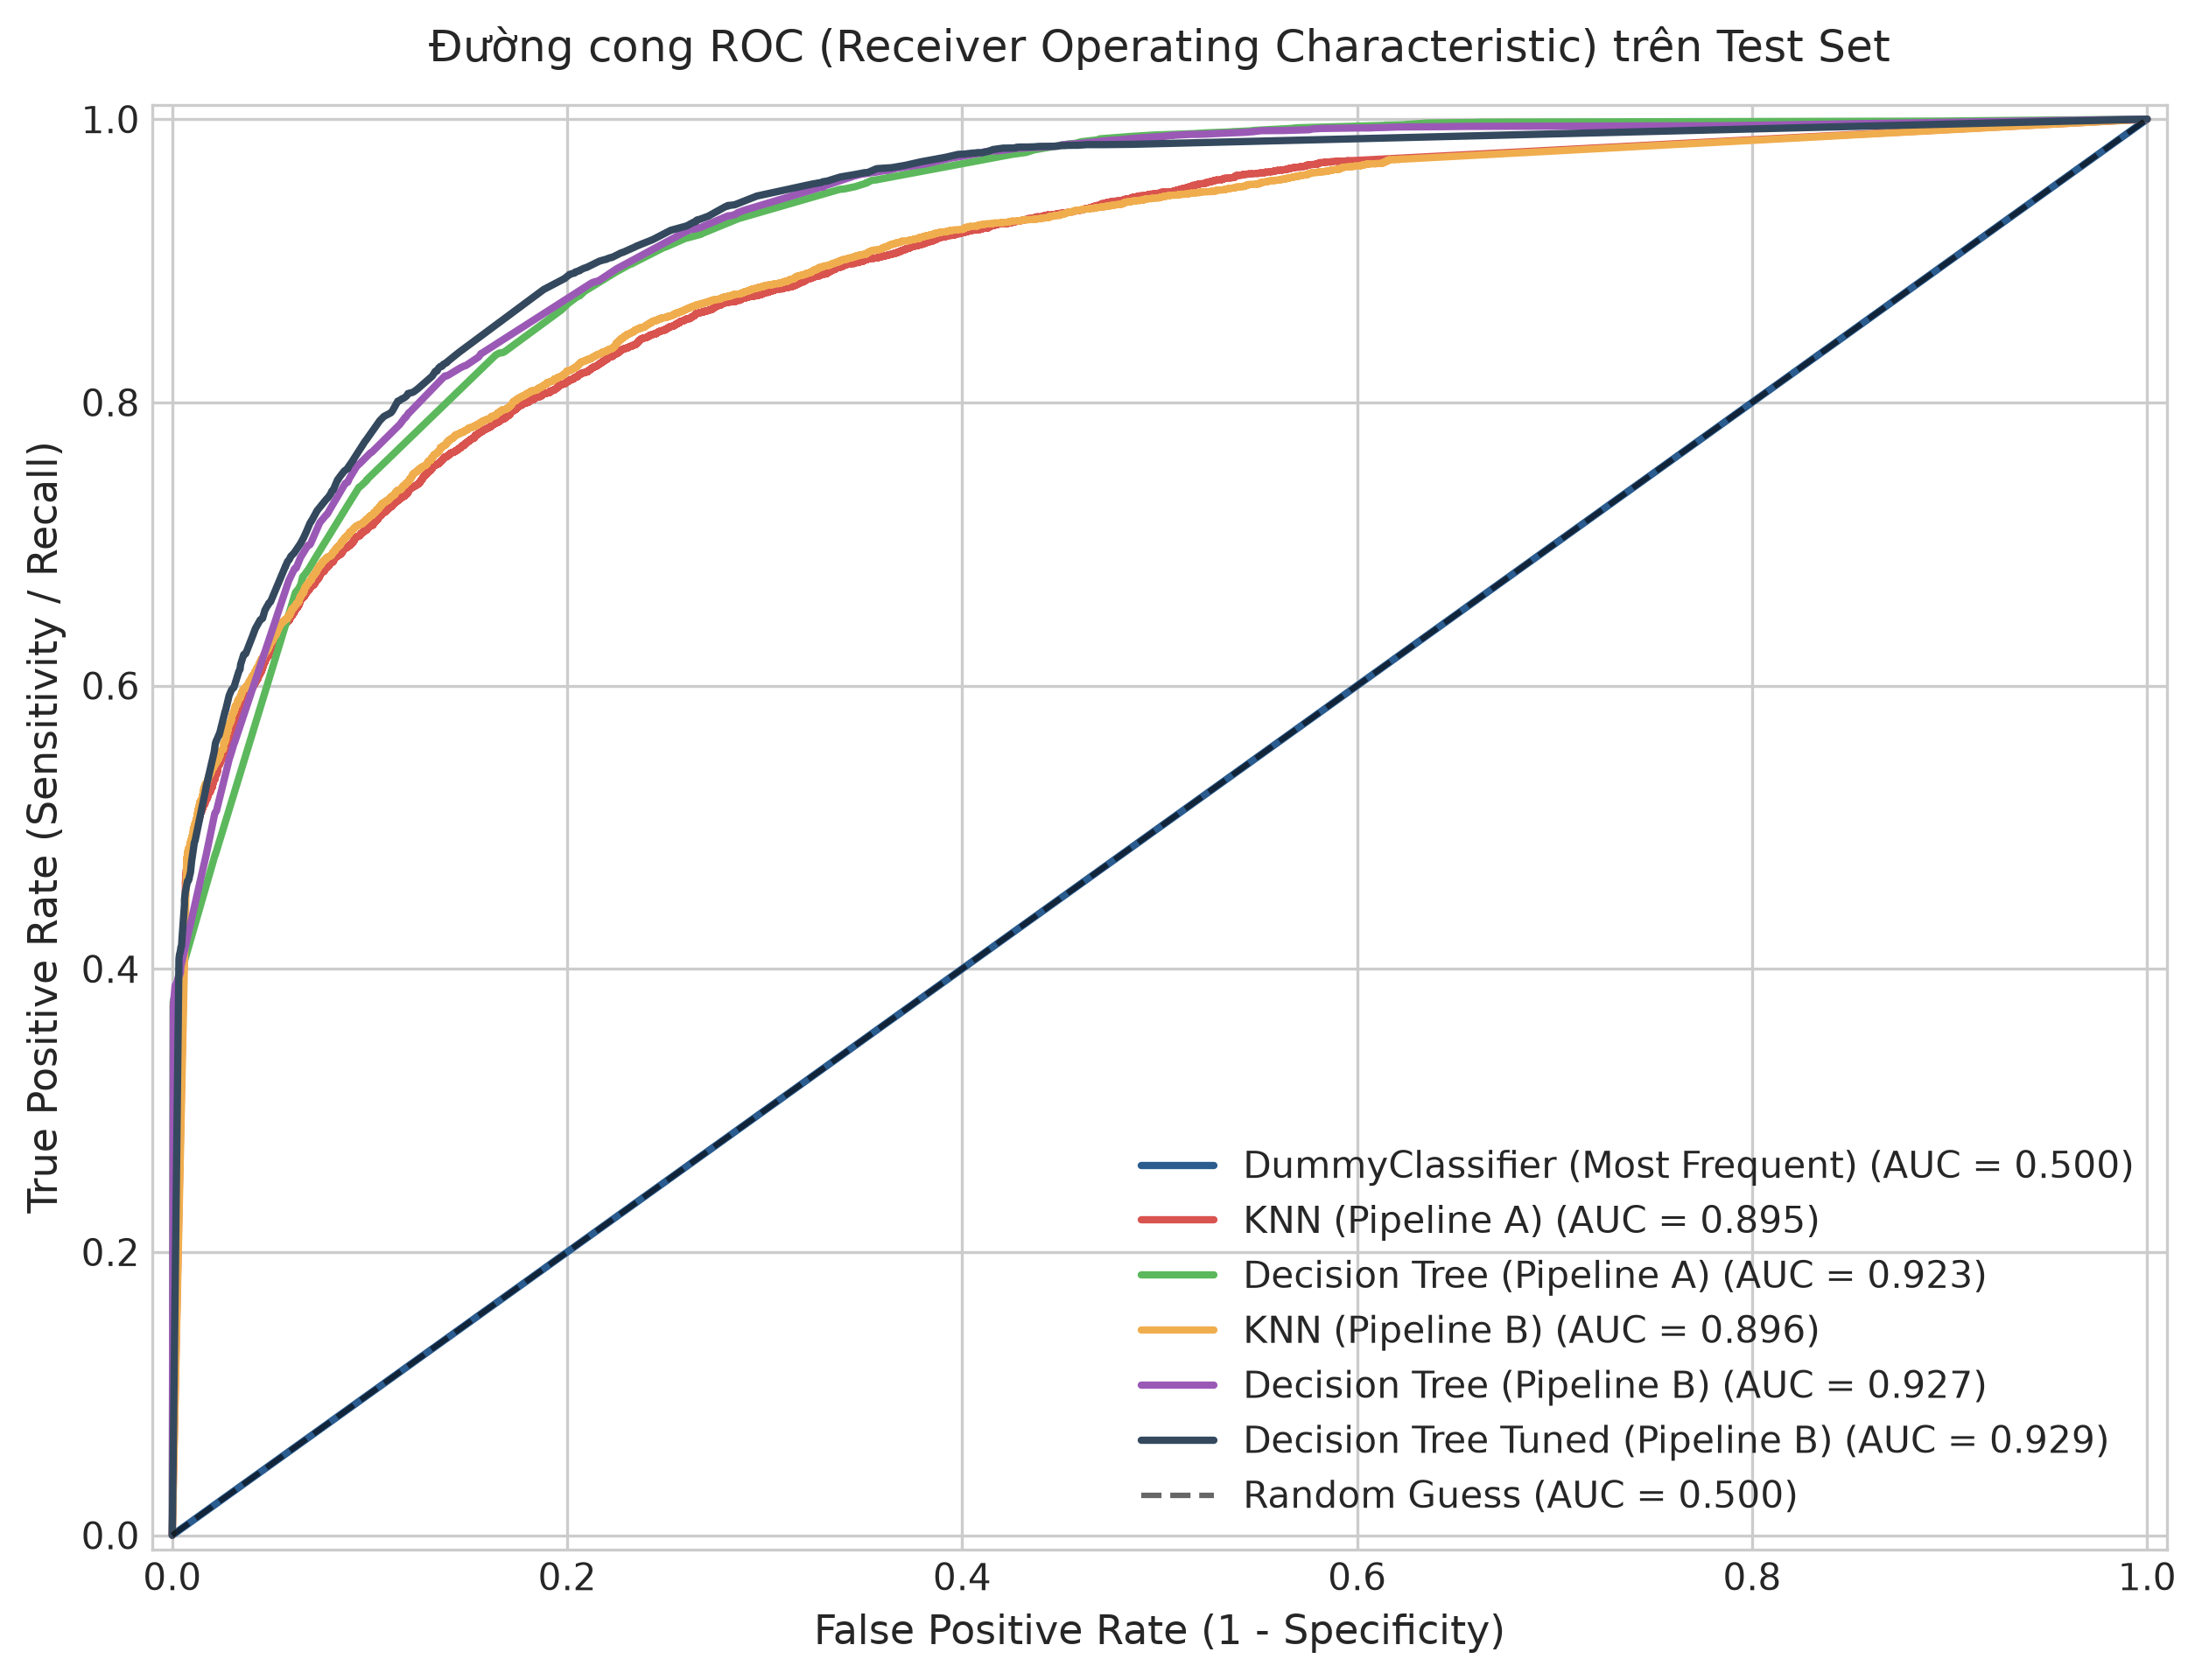
\includegraphics[width=\linewidth]{roc_curves_comparison.png}
        \caption{So sánh đường cong ROC}
    \end{subfigure}
    \begin{subfigure}{0.48\textwidth}
        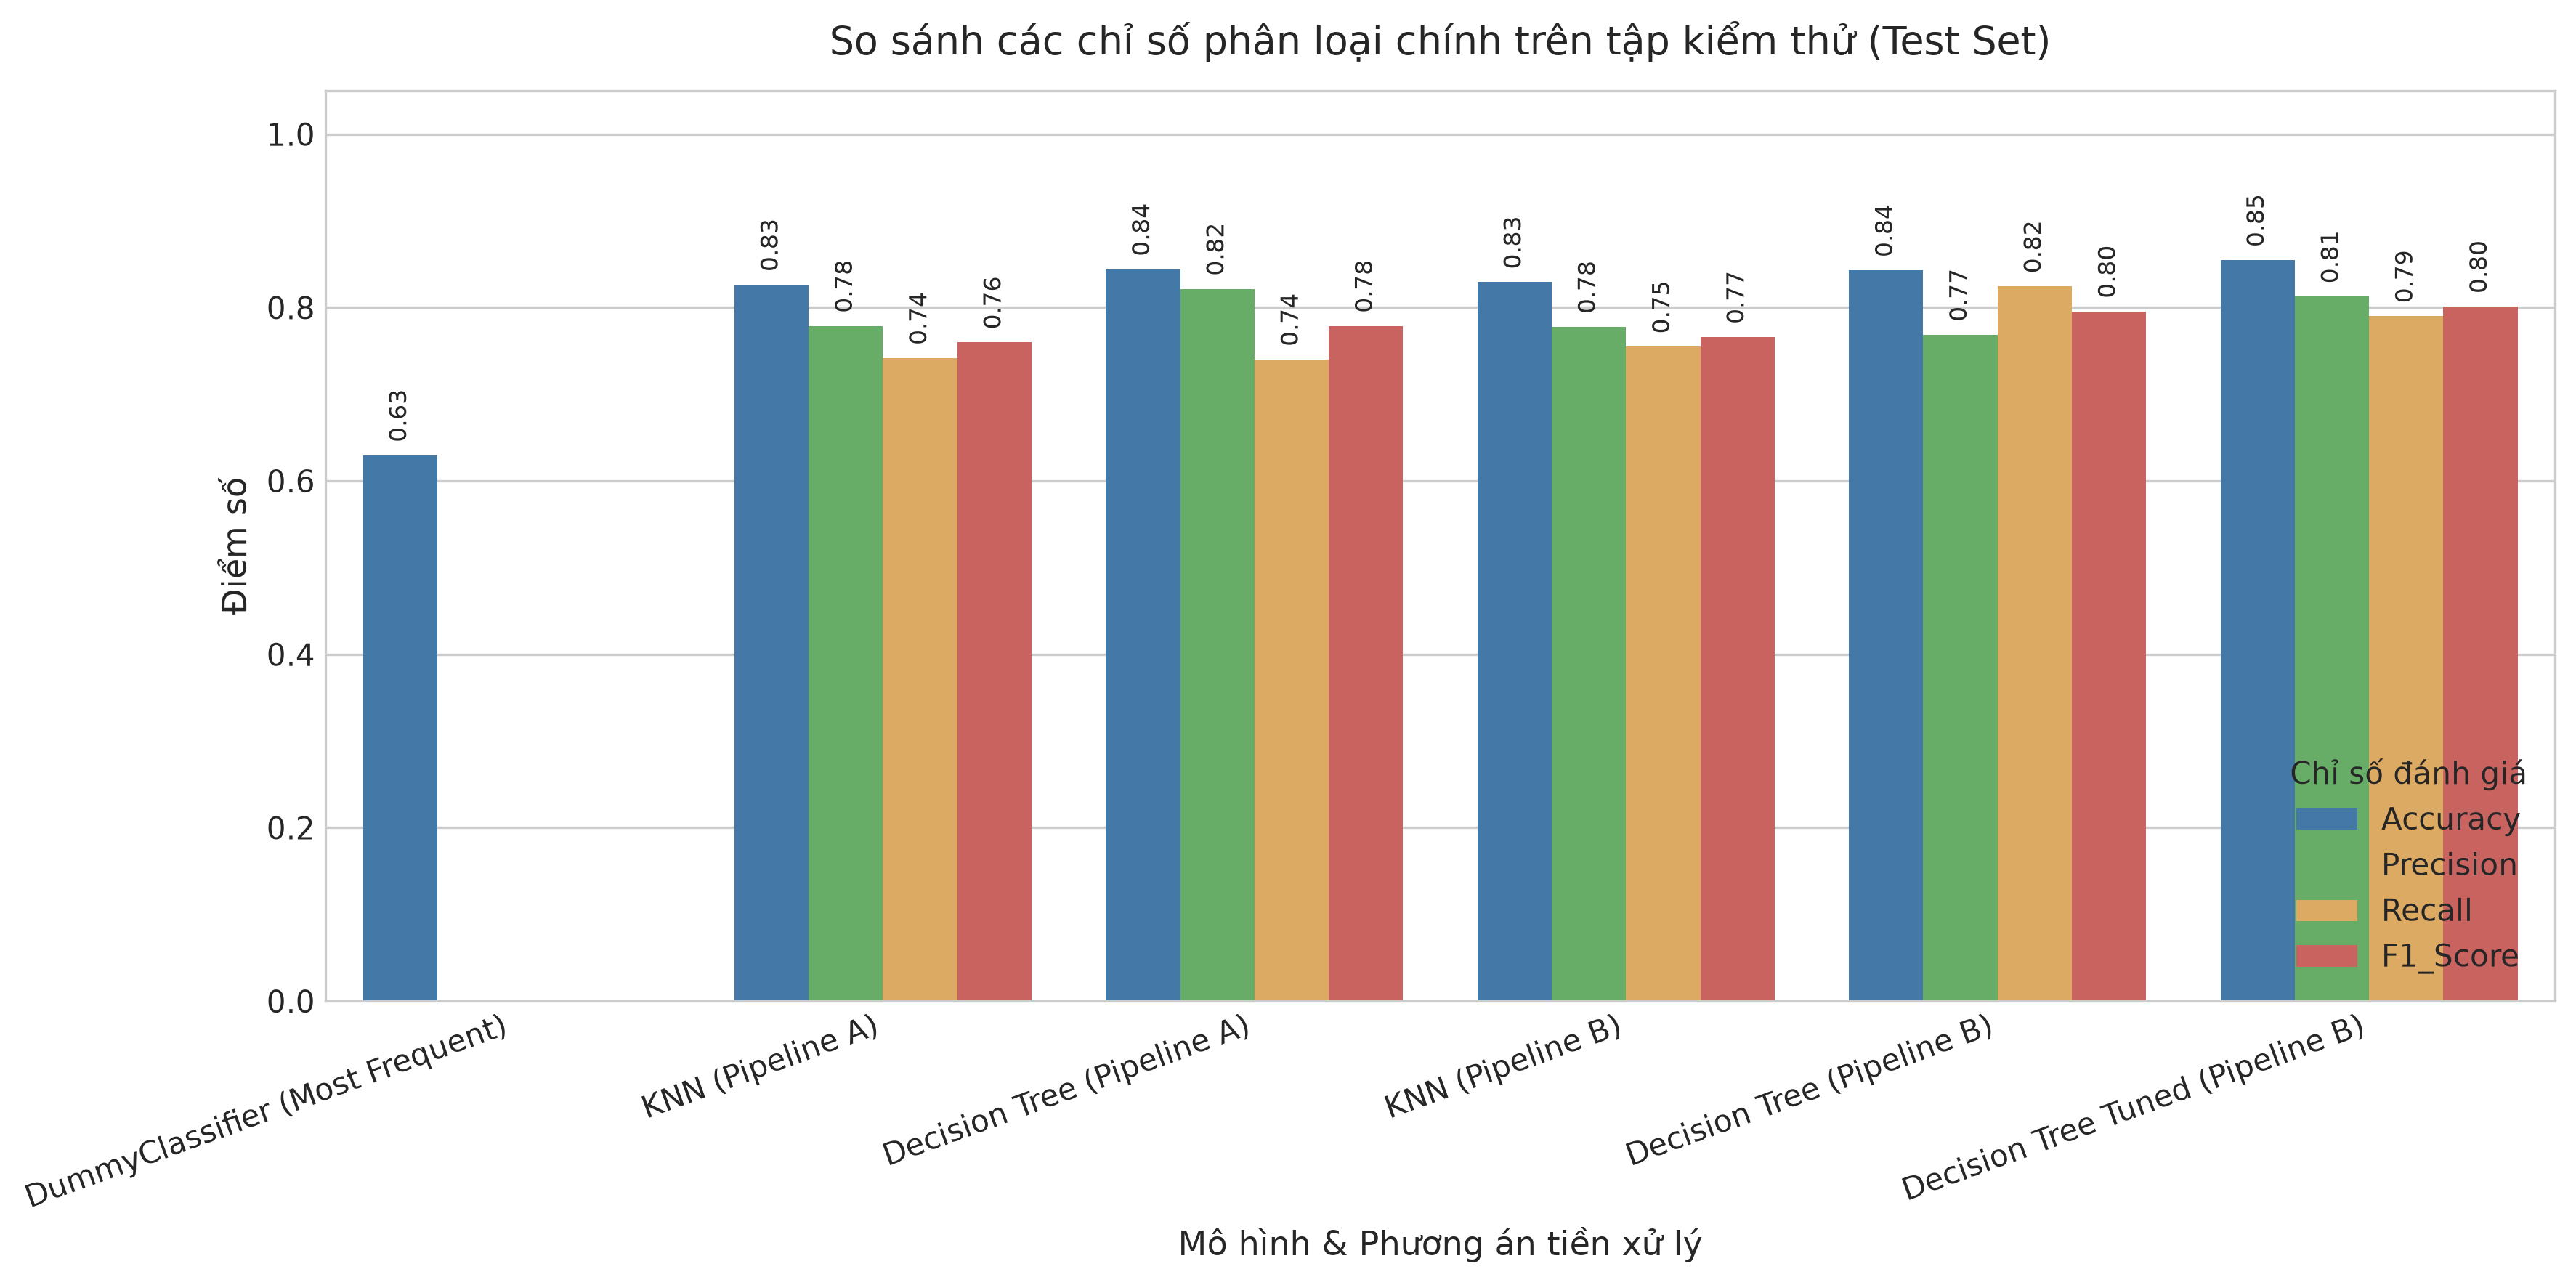
\includegraphics[width=\linewidth]{model_metrics_comparison.png}
        \caption{So sánh các chỉ số phân loại}
    \end{subfigure}
    \caption{Đánh giá trực quan hiệu năng các mô hình trên tập kiểm thử}
    \label{fig:model_evaluation}
\end{figure}

\begin{figure}[H]
    \centering
    \begin{subfigure}{0.48\textwidth}
        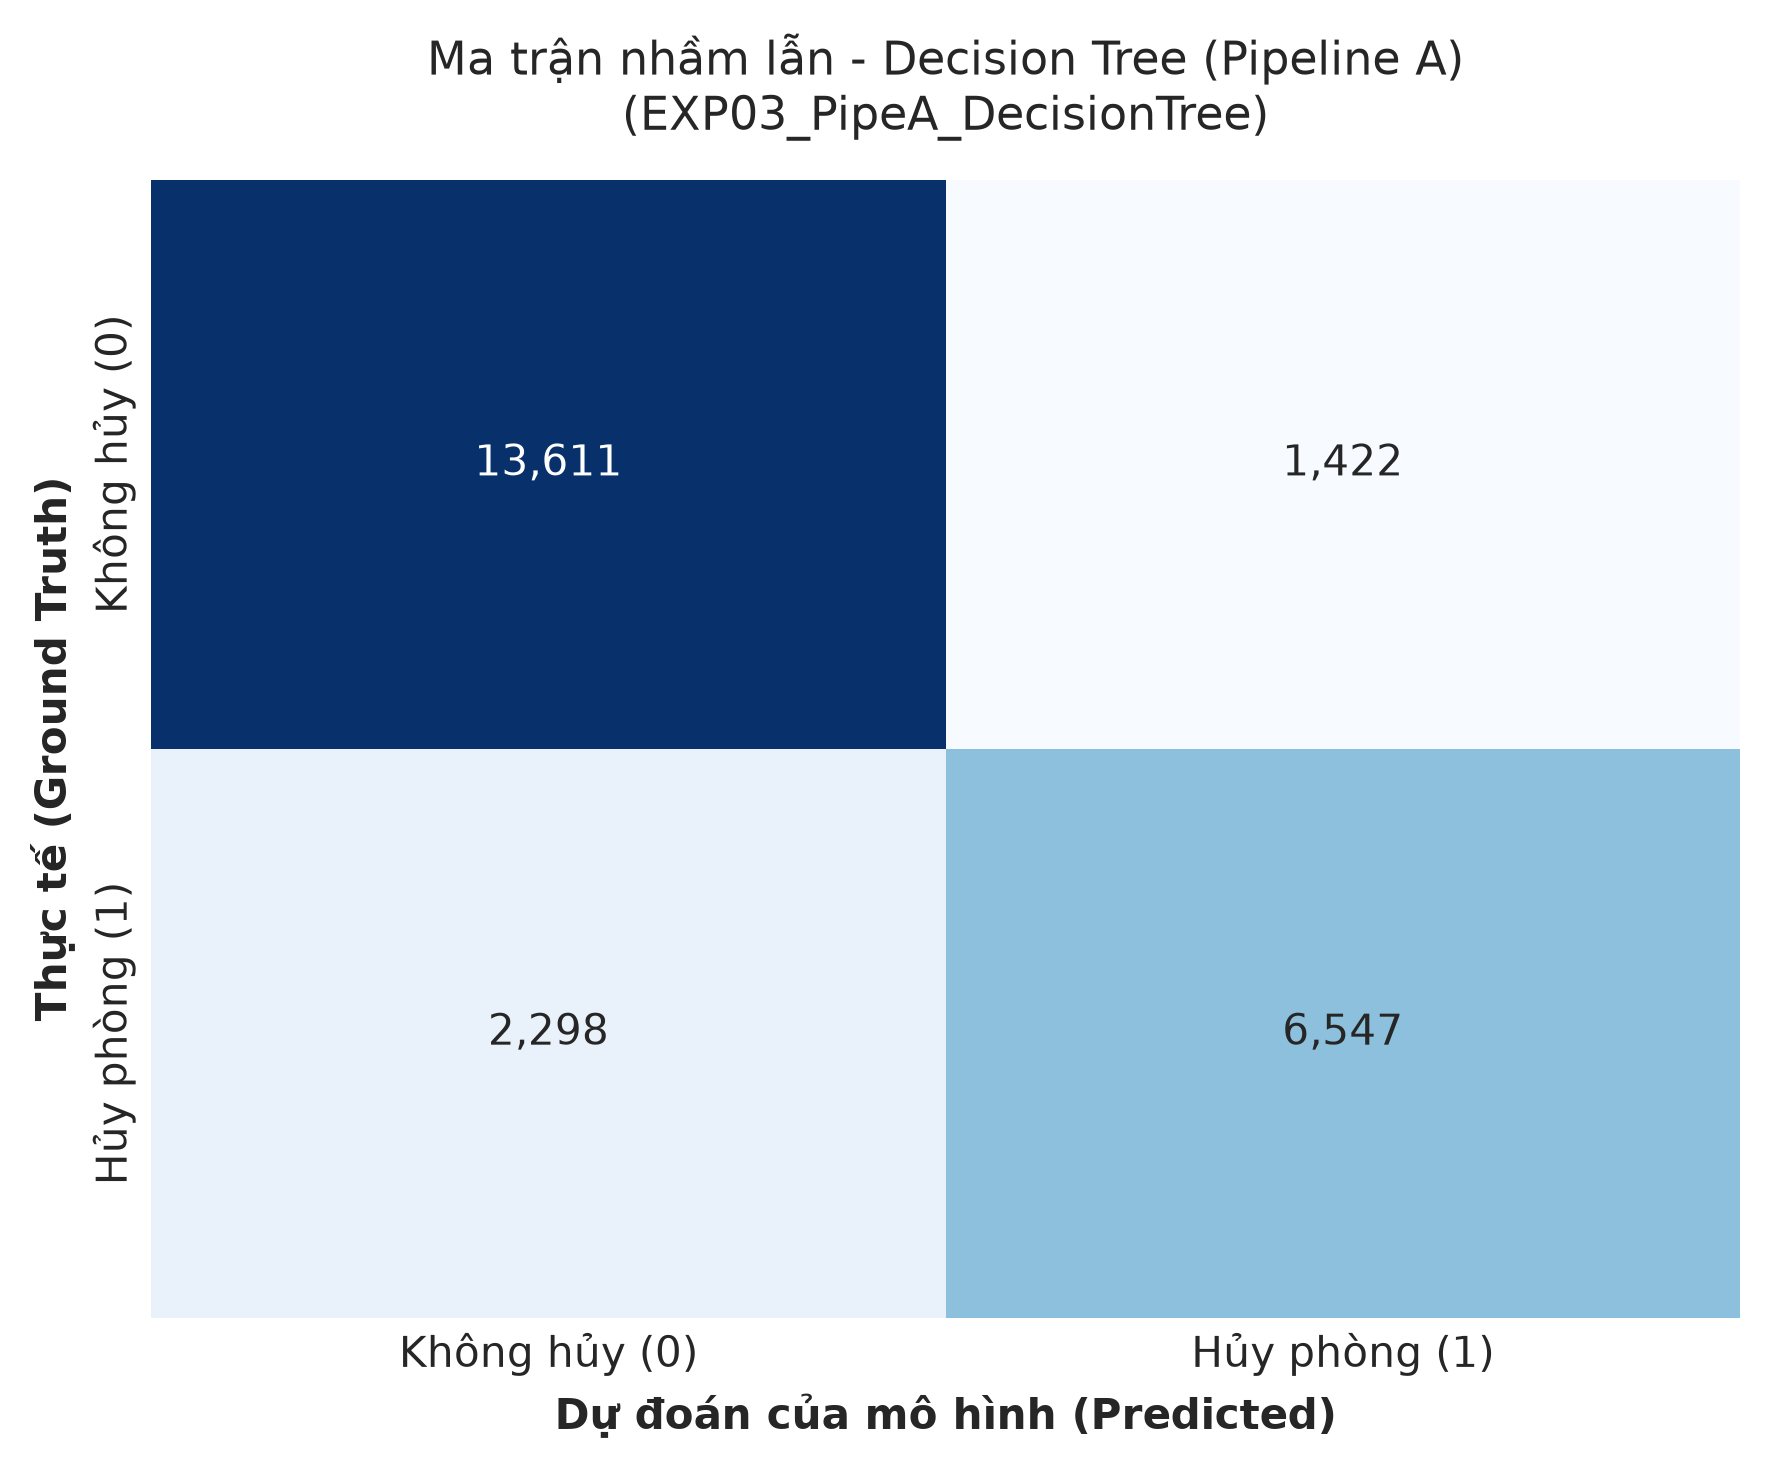
\includegraphics[width=\linewidth]{confusion_matrix_exp03_pipea_decisiontree.png}
        \caption{Ma trận nhầm lẫn EXP03 (DT Pipe A)}
    \end{subfigure}
    \begin{subfigure}{0.48\textwidth}
        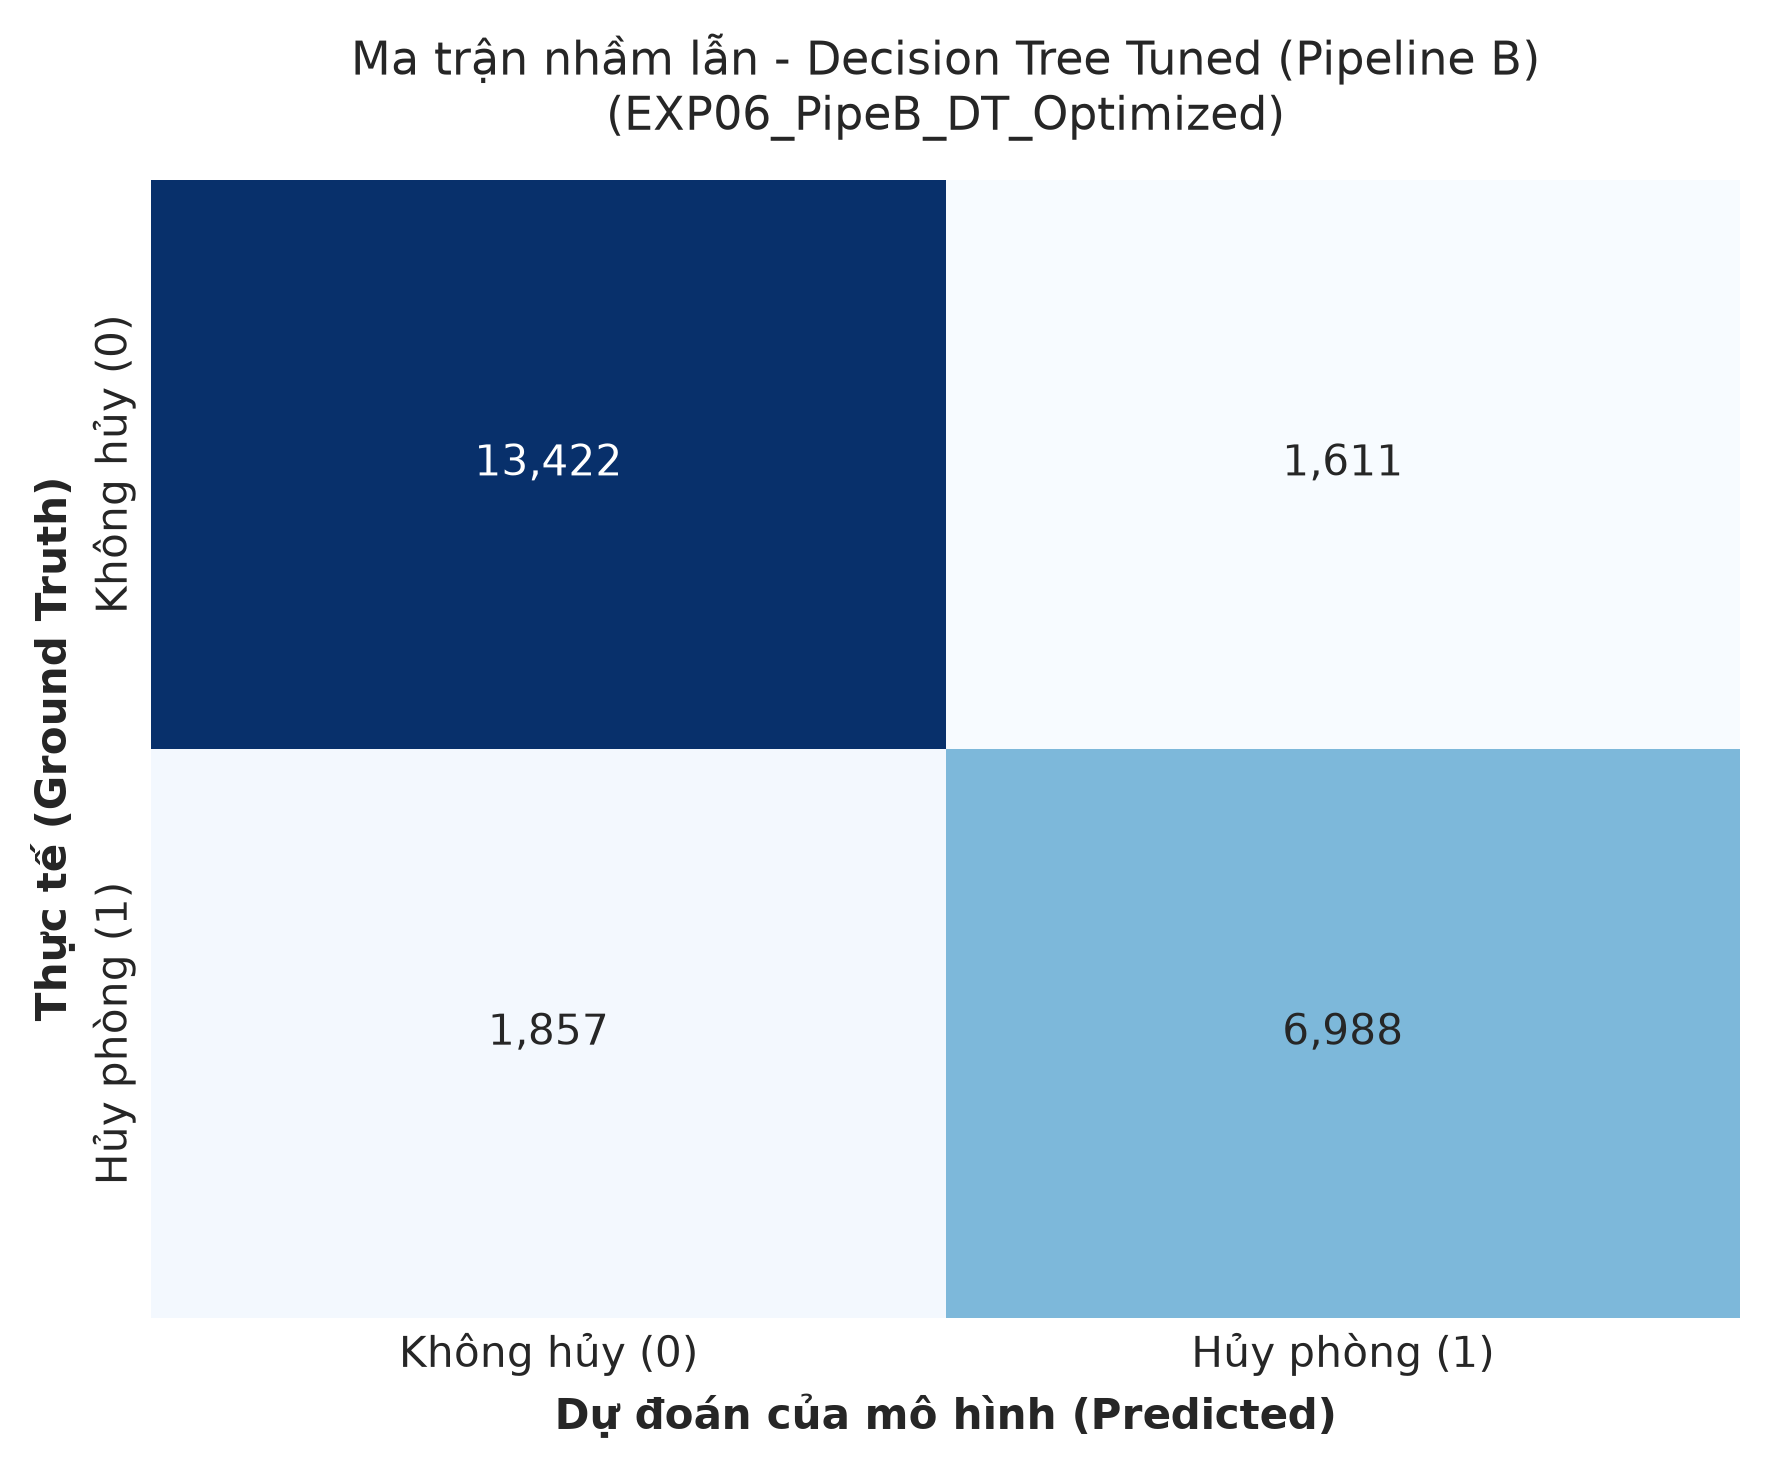
\includegraphics[width=\linewidth]{confusion_matrix_exp06_pipeb_dt_optimized.png}
        \caption{Ma trận nhầm lẫn EXP06 (DT Tuned Pipe B)}
    \end{subfigure}
    \caption{So sánh ma trận nhầm lẫn giữa Decision Tree trên Pipeline A và Pipeline B}
    \label{fig:confusion_matrices}
\end{figure}

\chapter{THẢO LUẬN VÀ SO SÁNH}

\section{So sánh hai phương án tiền xử lý (Pipeline A vs Pipeline B)}
Kết quả thực nghiệm đã chứng minh rõ ràng vai trò tích cực của kỹ thuật tiền xử lý cải tiến:
\begin{itemize}
    \item Đối với KNN: Pipeline B nâng Accuracy từ $82.63\%$ lên $82.93\%$, Recall tăng từ $74.18\%$ lên $75.48\%$ và F1-Score tăng từ $75.98\%$ lên $76.61\%$. Việc gom nhóm các quốc gia hiếm giúp giảm độ phân tán của không gian khoảng cách Euclid, trong khi chuẩn hóa \texttt{RobustScaler} làm giảm tác động của các giá trị ngoại lệ trong biến \texttt{lead\_time}.
    \item Đối với Decision Tree: Các đặc trưng phái sinh như \texttt{room\_type\_changed} (phòng bị đổi có tỷ lệ hủy chỉ $5.45\%$) và \texttt{is\_family} đã trở thành các điểm phân tách cực kỳ hữu ích ở các tầng trên cùng của cây quyết định.
\end{itemize}

\section{So sánh thuật toán KNN và Decision Tree}
\begin{itemize}
    \item \textbf{Về mặt hiệu năng:} Decision Tree vượt trội hoàn toàn so với KNN ở mọi chỉ số (F1-score $80.12\%$ so với $76.61\%$, ROC-AUC $0.9289$ so với $0.8965$).
    \item \textbf{Về chi phí tính toán:} Decision Tree có tốc độ huấn luyện và dự đoán rất nhanh ($O(d \cdot \text{depth})$ khi dự đoán), trong khi KNN đòi hỏi tính toán khoảng cách tới hàng chục nghìn điểm huấn luyện nên tốn thời gian và bộ nhớ hơn đáng kể.
    \item \textbf{Về khả năng giải thích (Interpretability):} Cây quyết định cung cấp cấu trúc quy tắc phân nhánh \textit{if-else} trực quan, giúp nhà quản trị khách sạn hiểu được lý do tại sao một đơn phòng bị dự đoán có nguy cơ hủy cao.
\end{itemize}

\section{Phân tích tương quan giữa Precision, Recall và F1-score}
Trong bài toán quản trị khách sạn, có một sự đánh đổi (Trade-off) rõ rệt giữa Precision và Recall:
\begin{itemize}
    \item \textbf{EXP03 (Cây quyết định tiêu chuẩn):} Đạt Precision cao ($82.16\%$) nhưng Recall chỉ đạt $74.02\%$. Khi mô hình cảnh báo hủy, độ tin cậy rất cao (ít báo động giả), nhưng lại bỏ sót tới 2,298 đơn đặt phòng bị hủy (False Negative).
    \item \textbf{EXP05 (Cây quyết định Balanced):} Khi điều chỉnh trọng số phạt mẫu hủy, Recall tăng vọt lên $82.44\%$ (giảm số đơn bỏ sót xuống chỉ còn 1,553 đơn), nhưng kéo theo Precision giảm xuống $76.87\%$.
    \item Tùy thuộc vào chính sách kinh doanh (mùa cao điểm hay mùa thấp điểm), khách sạn có thể lựa chọn mô hình thiên về Recall (để chuẩn bị phòng bán lại) hoặc thiên về Precision (để tránh làm phiền khách hàng thực sự đến ở).

\end{itemize}

\section{Phân tích chuyên sâu về False Positive (Báo động giả)}
Nhóm False Positive (1,611 mẫu, chiếm $6.75\%$ tập test) là những đơn phòng được mô hình dự đoán sẽ hủy, nhưng thực tế khách vẫn đến nhận phòng (Check-Out thành công).
\begin{itemize}
    \item \textbf{Nguyên nhân:} Các đơn này thường có thời gian đặt trước rất dài (\texttt{lead\_time} lớn), không có yêu cầu đặc biệt và đi theo hình thức đặt qua đại lý trực tuyến (Online TA) -- vốn là các đặc điểm trùng khớp với các mẫu đơn bị hủy thông thường.
    \item \textbf{Rủi ro nghiệp vụ:} Nếu khách sạn tự động bán chồng phòng (Overbooking) quá sớm đối với nhóm này, khi khách đến nhận phòng khách sạn sẽ rơi vào tình trạng thiếu phòng và phải chịu chi phí bồi thường đắt đỏ.
\end{itemize}

\section{Phân tích chuyên sâu về False Negative (Bỏ sót rủi ro)}
Nhóm False Negative (1,857 mẫu, chiếm $7.78\%$ tập test) là những đơn phòng mô hình dự đoán sẽ không hủy, nhưng thực tế khách đã hủy phòng đột xuất.
\begin{itemize}
    \item \textbf{Đặc điểm thống kê:}
    \begin{itemize}
        \item Thời gian đặt trước (\texttt{lead\_time}) rất ngắn: Trung bình chỉ \textbf{83.40 ngày}, so với \textbf{161.89 ngày} của nhóm True Positive (nhóm bắt trúng hủy phòng).
        \item $75.82\%$ ca False Negative xảy ra tại \textbf{City Hotel} (khách sạn nội đô).
    \end{itemize}
    \item \textbf{Nguyên nhân nghiệp vụ:} Khách công vụ hoặc khách lưu trú ngắn hạn tại thành phố thường đặt phòng sát ngày và hủy phòng đột xuất do lịch trình làm việc thay đổi vào phút chót. Hành vi này không để lại dấu hiệu cảnh báo trước trong dữ liệu đặt phòng ban đầu.
\end{itemize}

\begin{figure}[H]
    \centering
    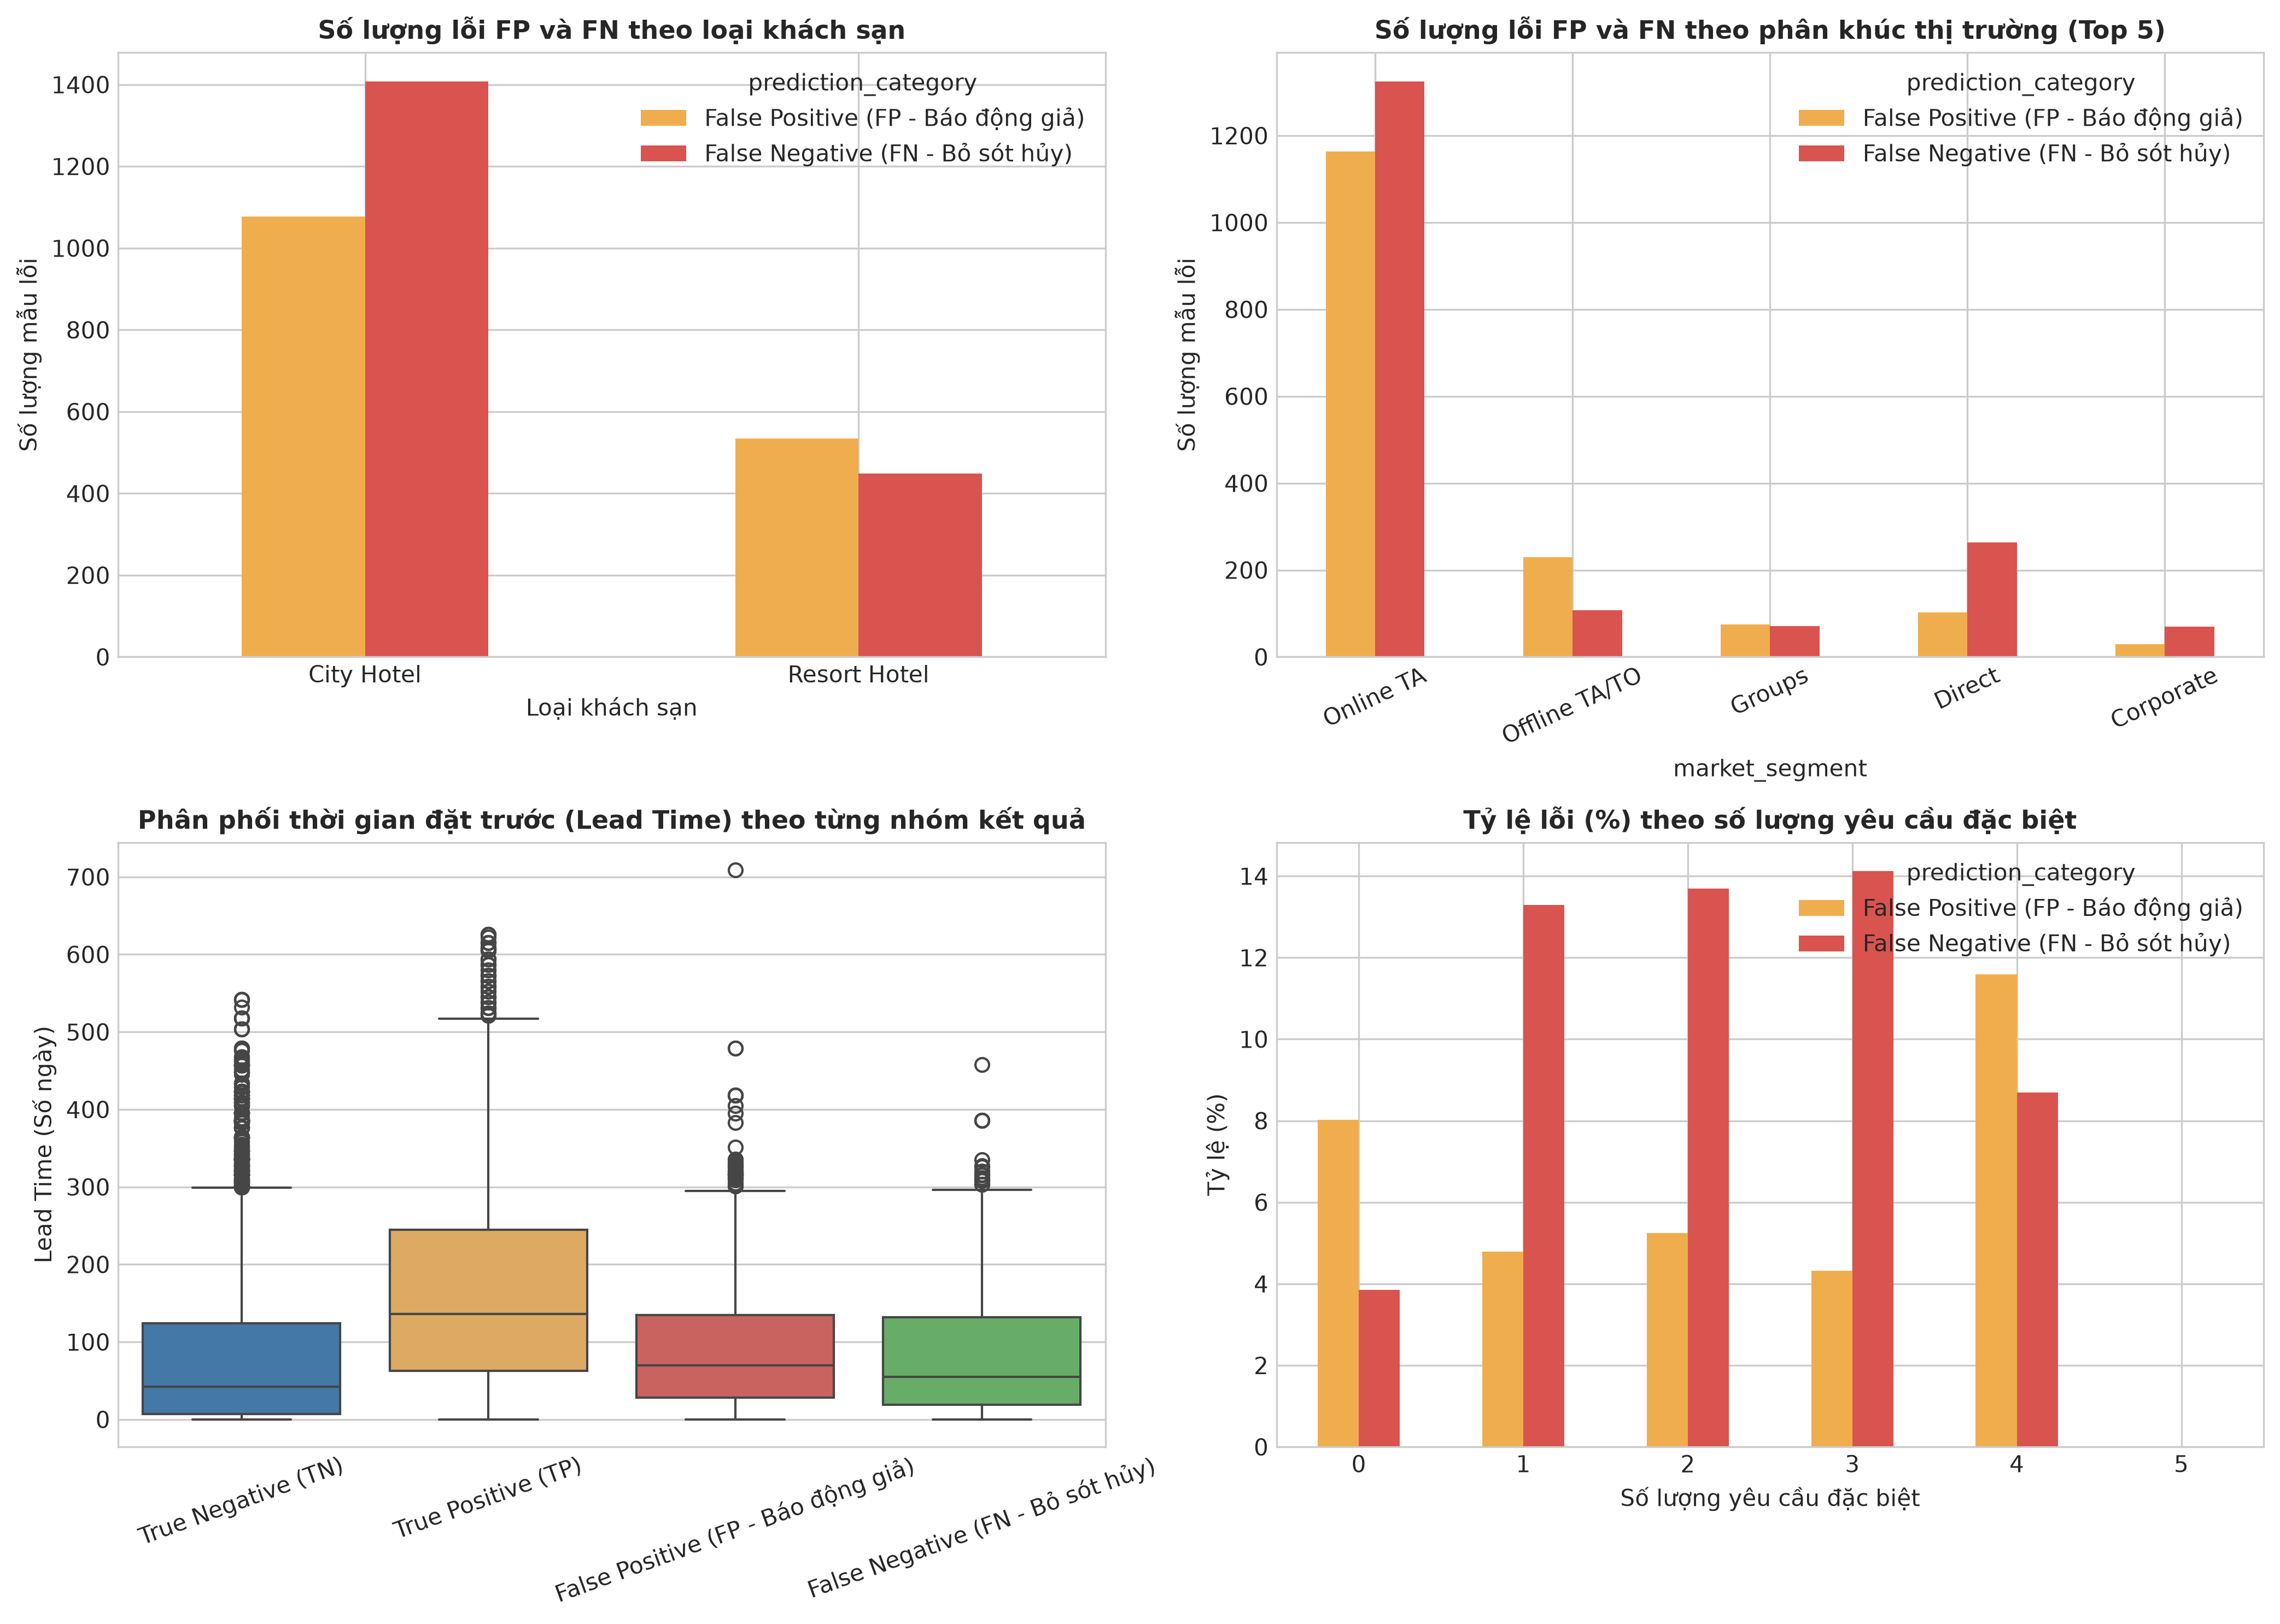
\includegraphics[width=0.9\linewidth]{error_analysis_breakdown.png}
    \caption{Phân bố lỗi False Positive và False Negative theo các đặc trưng nghiệp vụ}
    \label{fig:error_breakdown}
\end{figure}

\section{Hạn chế của dữ liệu và mô hình}
\begin{itemize}
    \item \textbf{Thiếu thông tin kinh tế vĩ mô và thời tiết:} Dữ liệu chưa tích hợp giá vé máy bay, yếu tố thời tiết hoặc các sự kiện lễ hội tại địa phương.
    \item \textbf{Dữ liệu ẩn danh:} Không có mã định danh khách hàng duy nhất để phân tích hành vi lịch sử dài hạn của từng cá nhân (Customer Lifetime Behavior).
    \item \textbf{Đặc thù thuật toán KNN:} KNN không phù hợp cho các hệ thống phục vụ trực tuyến quy mô lớn do chi phí bộ nhớ và độ trễ truy vấn cao.
\end{itemize}

\section{Khả năng ứng dụng thực tế trong quản trị khách sạn}
Mô hình tối ưu EXP06 có thể được tích hợp trực tiếp vào hệ thống Quản lý tài sản khách sạn (Property Management System -- PMS):
\begin{enumerate}
    \item \textbf{Định lượng tỷ lệ Overbooking động:} Dự báo chính xác số lượng phòng có nguy cơ bị hủy để khách sạn chủ động mở bán vượt mức tương ứng mà không sợ thiếu phòng.
    \item \textbf{Chính sách chăm sóc khách hàng chủ động:} Với các đơn đặt trước từ 3 tháng trở lên được cảnh báo có nguy cơ hủy, bộ phận lễ tân có thể gửi email xác nhận lịch trình, đề xuất giảm giá bữa ăn hoặc dịch vụ đưa đón để giữ chân khách hàng.
\end{enumerate}

\chapter{TỔNG KẾT VÀ HƯỚNG PHÁT TRIỂN}

\section{Tổng kết kết quả}
Dự án nghiên cứu đề tài 14 \textbf{``Dự đoán khách hàng hủy đặt phòng khách sạn''} đã hoàn thành toàn diện toàn bộ các mục tiêu đặt ra:
\begin{enumerate}
    \item Đã xây dựng quy trình phân tích và khai phá dữ liệu (EDA) chuẩn mực trên bộ dữ liệu \textit{Hotel Booking Demand} gồm 119,390 dòng quan sát, nhận diện các thuộc tính rủi ro hàng đầu (\texttt{lead\_time}, \texttt{deposit\_type}, \texttt{hotel}, \texttt{special\_requests}).
    \item Đã thiết kế thành công hai luồng tiền xử lý (Pipeline A và Pipeline B), thiết lập cơ chế kiểm soát chống rò rỉ dữ liệu (No Data Leakage) ở mức độ tuyệt đối.
    \item Đã tiến hành thử nghiệm, kiểm định chéo và đánh giá độc lập 6 mô hình học máy: Baseline (DummyClassifier), K-Nearest Neighbors (KNN) và Decision Tree.
    \item Đạt kết quả thực nghiệm tối ưu với mô hình Decision Tree trên Pipeline B: \textbf{Accuracy đạt 85.48\%, F1-Score đạt 80.12\% và ROC-AUC đạt 0.9289} trên tập kiểm thử độc lập 23,878 mẫu.
    \item Đã tiến hành chẩn đoán chuyên sâu các trường hợp lỗi False Positive và False Negative, giải thích tường minh cơ chế phát sinh lỗi dưới góc độ nghiệp vụ lưu trú.
\end{enumerate}

\section{Những nội dung đã hoàn thành}
\begin{itemize}
    \item Toàn bộ mã nguồn được module hóa hướng đối tượng chuẩn PEP 8 trong thư mục \texttt{src/}.
    \item Xây dựng hệ thống 5 Jupyter Notebooks có thể tái lập từ đầu đến cuối trong thư mục \texttt{notebooks/}.
    \item Bộ kiểm thử tự động (\texttt{pytest}) đạt tỷ lệ thành công 100\% (13/13 test cases passed).
    \item Xuất bản đầy đủ bảng biểu và đồ thị phân tích chất lượng cao vào thư mục \texttt{reports/}.
    \item Soạn thảo hoàn chỉnh báo cáo khoa học 6 chương bằng LaTeX và tài liệu thuyết minh dự án (\texttt{README.md}, \texttt{AI\_USAGE.md}, \texttt{docs/}).
\end{itemize}

\section{Hạn chế của nghiên cứu}
\begin{itemize}
    \item Nghiên cứu mới chỉ tập trung vào các thuật toán nền tảng trong chương trình học (KNN, Decision Tree), chưa triển khai các mô hình Ensemble học sâu (như Random Forest, Gradient Boosting).
    \item Mô hình chưa có dữ liệu phản hồi thời gian thực từ phía khách hàng (ví dụ: hành vi mở email xác nhận, lịch sử tương tác trên ứng dụng).
\end{itemize}

\section{Hướng phát triển trong tương lai}
\begin{enumerate}
    \item \textbf{Thử nghiệm các mô hình Ensemble:} Mở rộng thử nghiệm Random Forest, Extra Trees hoặc XGBoost để nâng cao hơn nữa chỉ số F1-Score.
    \item \textbf{Hiệu chỉnh xác suất (Probability Calibration):} Sử dụng Platt Scaling hoặc Isotonic Regression để biến đổi đầu ra của mô hình thành xác suất rủi ro được hiệu chuẩn chính xác, phục vụ tính toán giá trị kỳ vọng (Expected Monetary Value) trong tối ưu hóa doanh thu khách sạn.
    \item \textbf{Triển khai ứng dụng Web tương tác:} Hoàn thiện giao diện Streamlit cho phép nhân viên lễ tân nhập thông tin đặt phòng và nhận dự báo rủi ro hủy phòng tức thì.
\end{enumerate}

\chapter*{KHAI BÁO SỬ DỤNG TRỢ LÝ TRÍ TUỆ NHÂN TẠO}
\addcontentsline{toc}{chapter}{Khai báo sử dụng trợ lý Trí tuệ nhân tạo (AI Usage Statement)}

Nhóm sinh viên thực hiện đề tài xin cam kết tuân thủ nghiêm ngặt chuẩn mực về \textbf{Liêm chính học thuật (Academic Integrity)}. Quá trình thực hiện dự án có sử dụng công cụ trợ lý AI (Google Antigravity IDE / Gemini Models) với phạm vi minh bạch như sau:

\begin{enumerate}
    \item \textbf{Phạm vi hỗ trợ của AI:}
    \begin{itemize}
        \item Khởi tạo cấu trúc khung dự án phần mềm theo mô hình Machine Learning chuẩn mực.
        \item Gợi ý cú pháp định dạng mã nguồn Python tuân thủ chuẩn PEP 8 và mẫu định dạng văn bản khoa học LaTeX.
        \item Hỗ trợ cấu trúc các bài kiểm thử tự động (\texttt{pytest}) cho các module tiền xử lý dữ liệu.
    \end{itemize}
    \item \textbf{Cam đoan về tính xác thực của dữ liệu và kết quả thực nghiệm:}
    \begin{itemize}
        \item 100\% dữ liệu phân tích là bộ dữ liệu thực tế \textit{Hotel Booking Demand} của Jesse Mostipak. Tuyệt đối không sử dụng dữ liệu tự tạo giả định.
        \item Toàn bộ bảng số liệu đánh giá, ma trận nhầm lẫn và các đồ thị được sinh tự động và trung thực từ quá trình thực thi mã nguồn trên máy tính thực tế.
        \item Các diễn giải về nghiệp vụ lưu trú, phân tích tương quan và biện luận nguyên nhân lỗi được các thành viên trong nhóm trực tiếp nghiên cứu và đúc kết.
    \end{itemize}
\end{enumerate}

Nhóm sinh viên hoàn toàn chịu trách nhiệm về nội dung báo cáo và mã nguồn của dự án trước giảng viên hướng dẫn và hội đồng bảo vệ học phần.


% ==============================================================================
% TÀI LIỆU THAM KHẢO
% ==============================================================================
\newpage
\bibliographystyle{plain}
\bibliography{references}

\end{document}
